%%%%%%%%%%%%%%%%%%%%%%%%%%%%%%%%%%%%%%%%%%%%%%%%%%%%%%%%%%%%%%%%%%%%%%%%%%%%%%%
%                       DOCUMENT CLASS AND PACKAGES                         %
%%%%%%%%%%%%%%%%%%%%%%%%%%%%%%%%%%%%%%%%%%%%%%%%%%%%%%%%%%%%%%%%%%%%%%%%%%%%%%%

\documentclass[11pt,english]{report}

\usepackage[utf8]{inputenc} 
\usepackage{graphicx} 
\usepackage[english]{babel}
\usepackage{amsmath} 
\usepackage{booktabs} 
\usepackage{multirow}
\usepackage{float}
\usepackage{array}
\usepackage{tikz}
\usetikzlibrary{positioning, arrows.meta, calc, backgrounds, fit, shapes.geometric, matrix, chains}
\usepackage{pgfplots}
\pgfplotsset{compat=1.18}
\usepgfplotslibrary{groupplots}
\usepackage{natbib}            
\usepackage{pdfpages}
\usepackage{parskip}
\usepackage{tabularx}
\usepackage{subcaption}

\setlength{\parindent}{0pt}
\setlength{\parskip}{1em} 

%%%%%%%%%%%%%%%%%%%%%%%%%%%%%%%%%%%%%%%%%%%%%%%%%%%%%%%%%%%%%%%%%%%%%%%%%%%%%%%
%                 INFORMATION FOR THE COVER PAGE AND DOCUMENT               %
%%%%%%%%%%%%%%%%%%%%%%%%%%%%%%%%%%%%%%%%%%%%%%%%%%%%%%%%%%%%%%%%%%%%%%%%%%%%%%%

\newcommand{\theuniversity}{Universitat Politècnica de València}
\newcommand{\theschool}{DSIC - Departament de Sistemes Informàtics i Computació}
\newcommand{\thedegree}{MIARFID - Master's in Artificial Intelligence and Pattern Recognition}
\newcommand{\theprojecttype}{Academic Project}
\newcommand{\thetitle}{Optimization of Keyboard Layouts for English}
\newcommand{\theauthor}{Jordi Cantavella Ferrero}
\newcommand{\thecourse}{Academic Year 2025-2026}

%%%%%%%%%%%%%%%%%%%%%%%%%%%%%%%%%%%%%%%%%%%%%%%%%%%%%%%%%%%%%%%%%%%%%%%%%%%%%%%
%                              START OF DOCUMENT                              %
%%%%%%%%%%%%%%%%%%%%%%%%%%%%%%%%%%%%%%%%%%%%%%%%%%%%%%%%%%%%%%%%%%%%%%%%%%%%%%%
\usepackage[colorlinks=true, linkcolor=purple, citecolor=green!60!black, urlcolor=magenta]{hyperref}

\begin{document}

\begin{titlepage}
    \centering
    \vspace{1.5cm}
    {\Large \bfseries \theuniversity} \\
    \vspace{0.5cm}
    {\large \theschool} \\
    \vspace{2cm}
    {\large \textbf{\theprojecttype}} \\
    \vspace{0.2cm}
    {\large \thedegree} \\
    \vfill 
    {\Huge \bfseries \thetitle} \\
    \vfill
    \begin{minipage}{0.8\textwidth}
        \begin{flushleft}
            \large
            \textbf{Author:} \\
            \theauthor \\
            \vspace{1cm}
        \end{flushleft}
    \end{minipage}
    \vfill
    {\large \thecourse}
\end{titlepage}

\tableofcontents
\listoffigures
\listoftables
\cleardoublepage


%%%%%%%%%%%%%%%%%%%%%%%%%%%%%%%%%%%%%%%%%%%%%%%%%%%%%%%%%%%%%%%%%%%%%%%%%%%%%%%
%                    MAIN CONTENT STRUCTURE                                 %
%%%%%%%%%%%%%%%%%%%%%%%%%%%%%%%%%%%%%%%%%%%%%%%%%%%%%%%%%%%%%%%%%%%%%%%%%%%%%%%

\chapter{Introduction} \label{chpt:1}
\section{Context}
Most keyboard layouts we use today weren't designed with ergonomics or typing efficiency in mind. Instead, they come from the era of mechanical typewriters and haven't really kept up with how we actually type on modern devices.

Take QWERTY, for example. It was created back in 1873 for mechanical typewriters. The layout was meant to prevent the mechanical keys from jamming, not to make typing easier or faster. Research has shown that QWERTY causes unnecessary finger movements, which leads to tired hands and can even cause injuries over time.

This is why we've seen alternatives like Dvorak (from 1936) and Colemak (from 2006). These layouts tried to fix the problems by putting frequently used keys in easier-to-reach positions, reducing how much your fingers need to move, and making typing more comfortable overall.

\section{Objectives}
The main goal of this project is to optimize keyboard layouts to create arrangements that are both ergonomic and efficient. I'll do this by implementing two optimization algorithms: genetic algorithms and simulated annealing. These will explore different possible layouts and find the best ones based on how comfortable they are to use and how well they match actual language patterns.

The specific objectives are:

\begin{itemize}
    \item Implement a genetic algorithm for generating and evaluating different keyboard layouts.
    \item Implement a simulated annealing algorithm for the same problem.
    \item Define evaluation metrics that consider distance, hand alternation, and finger effort.
    \item Systematically analyze the impact of algorithm parameters on optimization performance.
    \item Compare the generated layouts with existing ones such as \textit{QWERTY}, \textit{Dvorak}, and \textit{Colemak}.
\end{itemize}

\section{Scope and Limitations}
Due to time and resource constraints, this work focuses on optimizing keyboard layouts specifically for English. I won't be looking at the physical implementation of keyboards or how they might work on different devices.

The optimization will also focus on the most common Latin alphabet layouts, including all 26 letters plus the most frequently used punctuation marks.

\chapter{Problem Description and Theoretical Framework} \label{chpt:2}

\section{History of Keyboard Layouts} \label{sec:historia_teclados}
The \textbf{QWERTY} keyboard, designed in 1873 by Christopher Latham Sholes, was created to prevent the keys of early mechanical typewriters from jamming by separating frequently used letter pairs. The \textbf{Dvorak} keyboard (1936) was scientifically designed to improve efficiency, reducing finger movement by up to 35\% compared to QWERTY. The \textbf{Colemak} keyboard (2006) represents a modern evolution that balances efficiency with ease of transition from QWERTY.

\begin{figure}[H]
    \centering
    \includegraphics[width=0.4\textwidth]{../figures/qwerty-dvorak-colemak.jpg}
    \caption{Comparison of the QWERTY, Dvorak, and Colemak keyboard layouts.}
    \label{fig:keyboard_layouts}
\end{figure}

\section{Problem Modeling} \label{sec:modelado_problema}
The keyboard layout optimization problem is modeled as a combinatorial optimization problem where the goal is to find the best arrangement of 30 characters (26 letters plus 4 punctuation marks: period, comma, semicolon, apostrophe) [a..z,.,;,' ], representing the genotype.

The phenotype is represented as a permutation of these characters arranged on a 3x10 grid to minimize typing cost, which makes it easier to visualize the keyboard layout and key positions.

\subsection{Individual Representation}
Each keyboard layout is represented as a permutation of 30 characters arranged in a standard grid structure:

\begin{center} 
    \begin{verbatim}
        0,  1,  2,  3,  4,  5,  6,  7,  8,  9      (Top Row)
        10, 11, 12, 13, 14, 15, 16, 17, 18, 19     (Home Row)
        20, 21, 22, 23, 24, 25, 26, 27, 28, 29     (Bottom Row)
    \end{verbatim}
\end{center}

Each position is assigned to a specific finger based on standard touch typing conventions. Figure \ref{fig:finger_mapping} illustrates the finger assignments across the keyboard grid.

\begin{figure}[htbp]
\centering
\definecolor{finger0}{RGB}{255, 99, 71}
\definecolor{finger1}{RGB}{255, 165, 0}
\definecolor{finger2}{RGB}{255, 215, 0}
\definecolor{finger3}{RGB}{50, 205, 50}

\begin{tikzpicture}[scale=0.75]
    \node at (5, 3.5) {\texttt{Finger Mapping Grid (3×10)}};
    \node at (2, 2.7) {\textbf{LEFT}};
    
    % Left Hand
    \fill[finger0] (0, 2) rectangle (1, 3); \node[white] at (0.5, 2.5) {0};
    \fill[finger1] (1, 2) rectangle (2, 3); \node[white] at (1.5, 2.5) {1};
    \fill[finger2] (2, 2) rectangle (3, 3); \node[white] at (2.5, 2.5) {2};
    \fill[finger3] (3, 2) rectangle (4, 3); \node[white] at (3.5, 2.5) {3};
    \fill[finger3] (4, 2) rectangle (5, 3); \node[white] at (4.5, 2.5) {4};
    
    \fill[finger0] (0, 1) rectangle (1, 2); \node[white] at (0.5, 1.5) {10};
    \fill[finger1] (1, 1) rectangle (2, 2); \node[white] at (1.5, 1.5) {11};
    \fill[finger2] (2, 1) rectangle (3, 2); \node[white] at (2.5, 1.5) {12};
    \fill[finger3] (3, 1) rectangle (4, 2); \node[white] at (3.5, 1.5) {13};
    \fill[finger3] (4, 1) rectangle (5, 2); \node[white] at (4.5, 1.5) {14};
    
    \fill[finger0] (0, 0) rectangle (1, 1); \node[white] at (0.5, 0.5) {20};
    \fill[finger1] (1, 0) rectangle (2, 1); \node[white] at (1.5, 0.5) {21};
    \fill[finger2] (2, 0) rectangle (3, 1); \node[white] at (2.5, 0.5) {22};
    \fill[finger3] (3, 0) rectangle (4, 1); \node[white] at (3.5, 0.5) {23};
    \fill[finger3] (4, 0) rectangle (5, 1); \node[white] at (4.5, 0.5) {24};
    
    \draw[very thick] (0, 0) rectangle (5, 3);
    \foreach \x in {1,2,3,4} \draw[thick] (\x, 0) -- (\x, 3);
    \foreach \y in {1,2} \draw[thick] (0, \y) -- (5, \y);
    
    \fill[gray!70] (5.15, -0.1) rectangle (5.35, 3.1);
    
    \node at (7.75, 2.7) {\textbf{RIGHT}};
    
    % Right Hand
    \fill[finger3] (5.5, 2) rectangle (6.5, 3); \node[white] at (6, 2.5) {5};
    \fill[finger3] (6.5, 2) rectangle (7.5, 3); \node[white] at (7, 2.5) {6};
    \fill[finger2] (7.5, 2) rectangle (8.5, 3); \node[white] at (8, 2.5) {7};
    \fill[finger1] (8.5, 2) rectangle (9.5, 3); \node[white] at (9, 2.5) {8};
    \fill[finger0] (9.5, 2) rectangle (10.5, 3); \node[white] at (10, 2.5) {9};
    
    \fill[finger3] (5.5, 1) rectangle (6.5, 2); \node[white] at (6, 1.5) {15};
    \fill[finger3] (6.5, 1) rectangle (7.5, 2); \node[white] at (7, 1.5) {16};
    \fill[finger2] (7.5, 1) rectangle (8.5, 2); \node[white] at (8, 1.5) {17};
    \fill[finger1] (8.5, 1) rectangle (9.5, 2); \node[white] at (9, 1.5) {18};
    \fill[finger0] (9.5, 1) rectangle (10.5, 2); \node[white] at (10, 1.5) {19};
    
    \fill[finger3] (5.5, 0) rectangle (6.5, 1); \node[white] at (6, 0.5) {25};
    \fill[finger3] (6.5, 0) rectangle (7.5, 1); \node[white] at (7, 0.5) {26};
    \fill[finger2] (7.5, 0) rectangle (8.5, 1); \node[white] at (8, 0.5) {27};
    \fill[finger1] (8.5, 0) rectangle (9.5, 1); \node[white] at (9, 0.5) {28};
    \fill[finger0] (9.5, 0) rectangle (10.5, 1); \node[white] at (10, 0.5) {29};
    
    \draw[very thick] (5.5, 0) rectangle (10.5, 3);
    \foreach \x in {6.5,7.5,8.5,9.5} \draw[thick] (\x, 0) -- (\x, 3);
    \foreach \y in {1,2} \draw[thick] (5.5, \y) -- (10.5, \y);
    
    % Legend
    \node[left] at (0, -1.15) {\textbf{Legend:}};
    \fill[finger0] (1, -0.9) rectangle (1.5, -1.4);
    \node[right] at (1.6, -1.15) {Pinky};
    \fill[finger1] (3.8, -0.9) rectangle (4.3, -1.4);
    \node[right] at (4.4, -1.15) {Ring};
    \fill[finger2] (6.6, -0.9) rectangle (7.1, -1.4);
    \node[right] at (7.2, -1.15) {Middle};
    \fill[finger3] (9.6, -0.9) rectangle (10.1, -1.4);
    \node[right] at (10.2, -1.15) {Index};
\end{tikzpicture}

\caption{Finger mapping visualization showing key-to-finger assignments.}
\label{fig:finger_mapping}
\end{figure}

\subsection{Fitness Function} \label{sec:fitness_function}
The fitness function evaluates typing cost by analyzing consecutive character pairs (bigrams) in the text. For each bigram, the cost is computed as:

\begin{equation}
    \text{cost}(c_i, c_{i+1}) = d_{\text{euclidean}}(c_i, c_{i+1}) \times \max(1.0 + P_{\text{finger}}(c_i, c_{i+1}), 0.1)
\end{equation}

where \textbf{$d_{\text{euclidean}}$} is the Euclidean distance between key positions and \textbf{$P_{\text{finger}}$} is a penalty system based on the following ergonomic factors:

\textbf{Same Finger Usage:} Heavy penalty (1.0) when consecutive characters use the same finger, with additional penalty (2.0) for weak fingers (pinky, ring).

\textbf{Same Hand Usage:} Moderate penalty (1.0) to promote hand alternation.

\textbf{Row Transitions:} Penalties for vertical movement (0.2 for adjacent rows, 0.8 for two-row jumps), with additional costs for weak fingers.

\textbf{Weak Finger Usage:} Penalties for pinky (0.15) and ring finger (0.1).

\textbf{Same Column Movement:} Extra penalty (0.3) for vertical movement, with additional costs for outer columns.

The total fitness is the sum of all bigram costs:

\begin{equation}
    F(\mathcal{L}) = \sum_{i=1}^{n-1} \text{cost}(c_i, c_{i+1})
\end{equation}

The objective is to \textbf{minimize $F(\mathcal{L})$}, resulting in layouts that reduce finger movement distance and optimize ergonomic factors.

\section{Linguistic Analysis and Datasets} \label{sec:datasets}
To analyze different text characteristics, this work uses two English literature corpora downloaded from Project Gutenberg:

\textbf{Moby Dick} by Herman Melville represents classical literature with rich, varied vocabulary and complex sentence structures, providing a comprehensive representation of formal English usage.

\textbf{The Wonderful Wizard of Oz} by L. Frank Baum represents children's literature with simpler vocabulary, repetitive phrasing, and straightforward sentence structures, reflecting common, everyday English patterns.

Each sample is pre-processed by converting all text to lowercase and removing all characters except the 30 included in our optimization (26 letters and 4 punctuation marks). Bigram frequencies are then computed for fitness evaluation.


\chapter{Genetic Algorithm: Methodology and Experiments} \label{chpt:3}

\section{Genetic Algorithm Implementation}

\subsection{Initial Population}
The population is initialized using a hybrid approach combining known layouts with random permutations. When using known distributions, the initial population includes QWERTY, Dvorak, QWERTZ, and Colemak layouts as starting points. The remaining individuals are randomly generated permutations, which helps maintain diversity for exploration.

\subsection{Selection: Tournament Selection}
The algorithm implements tournament selection with size $k$. In each tournament, $k$ individuals are randomly selected, and the one with the lowest fitness (best quality) becomes a parent. This process is repeated to select both parents for crossover. Tournament selection balances selection pressure (favoring good solutions) with diversity maintenance (allowing weaker solutions to participate).

\subsection{Crossover: Two-Point Crossover}
Two random crossover points divide parent layouts into segments. The child inherits a central segment from one parent and fills remaining positions from the other parent, ensuring valid permutations without duplicate characters. A duplicate-fixing function resolves any conflicts.

\subsection{Mutation: Swap Mutation}
Each individual has a certain probability of undergoing mutation. When mutation occurs, two random positions are selected and their characters are swapped. This simple operation maintains the permutation property while enabling local search.

\subsection{Replacement: Elitist Strategy}
The algorithm preserves the top percentage of individuals from the current generation and fills remaining slots with offspring from crossover and mutation. This ensures good solutions are never lost while allowing new genetic material to enter the population.

\section{Experimental Design} \label{sec:experimental_design}

To analyze the genetic algorithm's behavior and parameter sensitivity, four series of experiments were conducted. Each experiment varies one parameter while keeping all others constant, since running the full set of combinations would be computationally expensive.

The baseline configuration (Table \ref{tab:baseline_config}) was established based on preliminary experiments and computational constraints. Most experiments run for approximately 1.5 hours, and detailed results are available in the appendices (see Appendix \ref{appendix:ga_results} for complete GA experimental data).

\begin{table}[H]
    \centering
    \caption{Baseline Configuration for Parameter Experiments}
    \label{tab:baseline_config}
    \begin{tabular}{@{}ll@{}}
        \toprule
        \textbf{Parameter} & \textbf{Baseline Value} \\ 
        \midrule
        Population Size & 100,000 \\
        Generations & 150 \\
        Elite Rate & 15\% (15,000 individuals) \\
        Tournament Size & 5 \\
        Mutation Rate & 0.15 \\
        Random Seed & 123 \\
        \bottomrule
    \end{tabular}
\end{table}

\subsection{Experiment Series}
Four experiments were designed to evaluate the impact of key genetic algorithm parameters:

\textbf{Experiment 1: Population Size}\\
Population sizes tested: 1,000 - 10,000 - 100,000 - 1,000,000\\
This experiment evaluates how population size affects exploration capability and convergence speed.

\textbf{Experiment 2: Tournament Selection Size}\\
Tournament sizes ($k$) tested: 2 - 3 - 5 - 7 - 10\\
This experiment analyzes the balance between selection pressure and diversity maintenance.

\textbf{Experiment 3: Mutation Rate}\\
Mutation rates tested: 0.05 - 0.10 - 0.15 - 0.20 - 0.30 - 0.50 - 0.75\\
This experiment examines the role of mutation in maintaining diversity versus disrupting good solutions.

\textbf{Experiment 4: Elite Percentage}\\
Elite rates tested: 5\% - 10\% - 15\% - 20\% - 30\% - 50\%\\
This experiment investigates the trade-off between preserving best solutions and allowing population renewal.

Each experiment was run on both corpora (Moby Dick and Wizard of Oz) to assess corpus-specific effects.

\section{Experimental Results and Analysis}

\subsection{Experiment 1: Population Size}

Figure \ref{fig:exp1_population} shows the convergence curves for different population sizes on both corpora.

\begin{figure}[H]
    \centering
    \begin{subfigure}[b]{0.48\textwidth}
        \centering
        \includegraphics[width=\textwidth]{../figures/exp1_population_size_moby_dick.pdf}
        \caption{Moby Dick}
    \end{subfigure}
    \hfill
    \begin{subfigure}[b]{0.48\textwidth}
        \centering
        \includegraphics[width=\textwidth]{../figures/exp1_population_size_wonderful_wizard_oz.pdf}
        \caption{Wizard of Oz}
    \end{subfigure}
    \caption{Experiment 1: Impact of Population Size on convergence}
    \label{fig:exp1_population}
\end{figure}

\textbf{Key Observations:}

Small populations (1,000) show rapid initial convergence but achieve poor final fitness due to premature convergence and limited diversity.

Medium populations (10,000) provide a good balance between exploration and computational cost.

Large populations (100,000) achieve the best final fitness values, demonstrating superior exploration capability.

Very large populations (1,000,000) show only marginal improvement over 100,000 but with significantly higher computational cost.

\textbf{Corpus Differences:}
The simpler Wizard of Oz corpus shows less sensitivity to population size, with smaller populations achieving relatively good results. The complex Moby Dick corpus benefits more from larger populations, which suggests that complex linguistic landscapes require more extensive exploration.

\textbf{Conclusion:}
Population size of 100,000 provides the optimal balance between solution quality and computational efficiency for both corpora.

\subsection{Experiment 2: Tournament Selection Size}

Figure \ref{fig:exp2_tournament} illustrates the effect of tournament size on algorithm performance.

\begin{figure}[H]
    \centering
    \begin{subfigure}[b]{0.48\textwidth}
        \centering
        \includegraphics[width=\textwidth]{../figures/exp2_tournament_selection_moby_dick.pdf}
        \caption{Moby Dick}
    \end{subfigure}
    \hfill
    \begin{subfigure}[b]{0.48\textwidth}
        \centering
        \includegraphics[width=\textwidth]{../figures/exp2_tournament_selection_wonderful_wizard_oz.pdf}
        \caption{Wizard of Oz}
    \end{subfigure}
    \caption{Experiment 2: Impact of Tournament Selection Size}
    \label{fig:exp2_tournament}
\end{figure}

\textbf{Key Observations:}

Small tournaments ($k$=2) provide lower selection pressure and slower convergence.

Medium tournaments ($k$=3-5) offer optimal balance between exploration and exploitation.

Large tournaments ($k$=7-10) create strong selection pressure with faster initial convergence but risk premature convergence and getting stuck in local optima.

\textbf{Corpus Differences:}
Both corpora show similar patterns, with $k$=5 providing the best performance. However, the Wizard of Oz corpus is more forgiving, with less performance degradation for suboptimal tournament sizes.

\textbf{Conclusion:}
Tournament size $k$=5 provides the best balance for both corpora, offering strong enough selection pressure while maintaining sufficient diversity.

\subsection{Experiment 3: Mutation Rate}

Figure \ref{fig:exp3_mutation} demonstrates how mutation rate affects algorithm dynamics.

\begin{figure}[H]
    \centering
    \begin{subfigure}[b]{0.48\textwidth}
        \centering
        \includegraphics[width=\textwidth]{../figures/exp3_mutation_rate_moby_dick.pdf}
        \caption{Moby Dick}
    \end{subfigure}
    \hfill
    \begin{subfigure}[b]{0.48\textwidth}
        \centering
        \includegraphics[width=\textwidth]{../figures/exp3_mutation_rate_wonderful_wizard_oz.pdf}
        \caption{Wizard of Oz}
    \end{subfigure}
    \caption{Experiment 3: Impact of Mutation Rate}
    \label{fig:exp3_mutation}
\end{figure}

\textbf{Key Observations:}

Low mutation (0.05-0.10) leads to insufficient diversity and risk of stagnation.

Moderate mutation (0.15-0.20) provides optimal performance, maintaining diversity without excessive disruption.

High mutation (0.30-0.75) causes excessive disruption of good solutions, leading to slower convergence and worse final fitness.

\textbf{Corpus Differences:}
The Moby Dick corpus shows more sensitivity to mutation rate, with high mutation rates causing significant performance degradation. The Wizard of Oz corpus is more robust to varying mutation rates.

\textbf{Conclusion:}
Mutation rate of 0.15 provides optimal performance for both corpora, effectively balancing exploration through diversity maintenance and exploitation of good solutions.

\subsection{Experiment 4: Elite Percentage}

Figure \ref{fig:exp4_elite} shows the impact of elite preservation on algorithm performance.

\begin{figure}[H]
    \centering
    \begin{subfigure}[b]{0.48\textwidth}
        \centering
        \includegraphics[width=\textwidth]{../figures/exp4_elite_percentage_moby_dick.pdf}
        \caption{Moby Dick}
    \end{subfigure}
    \hfill
    \begin{subfigure}[b]{0.48\textwidth}
        \centering
        \includegraphics[width=\textwidth]{../figures/exp4_elite_percentage_wonderful_wizard_oz.pdf}
        \caption{Wizard of Oz}
    \end{subfigure}
    \caption{Experiment 4: Impact of Elite Percentage}
    \label{fig:exp4_elite}
\end{figure}

\textbf{Key Observations:}

Low elite rate (5\%) risks losing good solutions and shows slower convergence.

Moderate elite rate (10-20\%) provides optimal performance, preserving good solutions while allowing sufficient population renewal.

High elite rate (30-50\%) reduces diversity, leading to slower improvement and premature convergence.

\textbf{Corpus Differences:}
The Moby Dick corpus benefits from moderate elite rates (15-20\%), while the Wizard of Oz corpus performs well across a broader range (10-30\%), suggesting simpler optimization landscapes are more forgiving.

\textbf{Conclusion:}
Elite rate of 15\% provides the best balance for both corpora, ensuring preservation of high-quality solutions while maintaining sufficient population diversity for continued exploration.

\subsection{Summary of Parameter Experiments}

Table \ref{tab:optimal_parameters} summarizes the optimal parameter values identified through systematic experimentation.

\begin{table}[H]
    \centering
    \caption{Optimal Parameter Configuration}
    \label{tab:optimal_parameters}
    \begin{tabular}{@{}lll@{}}
        \toprule
        \textbf{Parameter} & \textbf{Optimal Value} & \textbf{Rationale} \\ 
        \midrule
        Population Size & 100,000 & Best exploration without excessive cost \\
        Tournament Size & 5 & Optimal selection pressure \\
        Mutation Rate & 0.15 & Balance diversity and exploitation \\
        Elite Rate & 15\% & Preserve quality, maintain diversity \\
        \bottomrule
    \end{tabular}
\end{table}

\textbf{General Findings:}

The Moby Dick corpus consistently requires more careful parameter tuning due to its complex linguistic structure.

The Wizard of Oz corpus is more forgiving across parameter ranges, suggesting simpler optimization landscapes.

All experiments confirm the importance of balancing exploration (diversity) and exploitation (convergence to good solutions).

The optimal parameters identified are consistent across both corpora, demonstrating robustness.

After reviewing all the genetic algorithm experiments on both corpora, we can draw some general conclusions about its performance and behavior. The choice of parameters significantly impacts the optimization process, with different settings working better for different corpora.

For Moby Dick, there's a clear need for more conservative parameter settings to avoid overfitting and ensure robust performance. This is likely because the text contains a larger number of bigrams, creating a more complex search space that better represents underlying language patterns with a more balanced distribution across different bigrams.

On the other hand, the Wizard of Oz corpus benefits from more diverse parameter settings, allowing greater flexibility in parameter tuning with a wider range of effective configurations. This corpus requires more exploration, as we can see with parameters like population size (1,000,000), tournament size (10), mutation rate (5\%), and elitism rate (5\%). This suggests the optimization process for this corpus works better with more exploration and population diversity. While Moby Dick needs less exploration and a more focused search strategy, the Wizard of Oz corpus thrives on broader exploration of the solution space. Overall, the GA parameters and experiments demonstrate the explorative nature of the optimization process.

\chapter{Simulated Annealing: Methodology and Experiments} \label{chpt:4}

\section{Simulated Annealing Algorithm}

Simulated Annealing (SA) is a probabilistic optimization technique inspired by the annealing process in metallurgy. When metals are heated and then slowly cooled, their atoms settle into low-energy configurations, reducing defects. SA mimics this physical process to solve optimization problems by gradually reducing the "temperature" parameter, which controls the algorithm's willingness to accept worse solutions.

The algorithm starts with a high temperature that allows exploration of the solution space by accepting both better and worse solutions. As the temperature decreases, the algorithm becomes more selective, eventually converging to a local (or ideally global) optimum. This balance between exploration and exploitation makes SA particularly effective for complex optimization problems like keyboard layout design.

\subsection{Initial Solution}

The algorithm can start from different initial configurations. For this work, I tested three categories of starting points. First, traditional layouts including QWERTY (the most common layout), Dvorak (a scientifically designed ergonomic layout), QWERTZ (the German variant of QWERTY), and Colemak (a modern efficiency-focused layout). Second, a completely random permutation of the 30 characters. Third, GA-optimized layouts from the previous chapter, including the best solutions from each of the four GA experiments (Exp1-4) plus the overall best layout from each corpus.

\subsection{Neighbor Generation}

Two neighborhood strategies control how the algorithm explores the solution space. Random Swap selects two random positions uniformly from all 30 positions and swaps their characters. This provides global exploration capability, allowing the algorithm to make large jumps in the solution space and escape local optima. Local Swap selects a random position and swaps it with one of its adjacent neighbors (left, right, top, or bottom in the 3×10 grid). This provides local refinement capability, making small adjustments that preserve most of the current solution's structure while fine-tuning its quality.

\subsection{Temperature Schedule}

The temperature $T$ controls the probability of accepting worse solutions. Three different cooling schedules were implemented to explore different exploration-exploitation trade-offs.

Geometric (Exponential) Cooling uses the formula $T(t) = T_0 \cdot k^t$, where $T_0$ is the initial temperature, $k \in (0, 1)$ is the cooling factor, and $t$ is the iteration number. This is the most commonly used schedule and provides exponential decay of temperature over time.

Logarithmic Cooling uses the formula $T(t) = \frac{T_0}{1 + k \cdot T_0 \cdot t}$. This schedule cools more slowly, especially early in the search, and provides theoretical guarantees of convergence to the global optimum under certain conditions.

Linear Cooling uses the formula $T(t) = \max(T_0 - k \cdot t, 0.01)$. This schedule provides uniform temperature decrease with a minimum threshold to prevent division by zero.

\subsection{Acceptance Criterion}

The algorithm uses the Metropolis acceptance criterion. For a candidate solution $S'$ with fitness $f(S')$ and current solution $S$ with fitness $f(S)$:

\begin{equation}
P(\text{accept}) = \begin{cases}
    1 & \text{if } \Delta f = f(S) - f(S') > 0 \text{ (improvement)} \\
    e^{\Delta f / T} & \text{if } \Delta f \leq 0 \text{ (worsening)}
\end{cases}
\end{equation}

Better solutions are always accepted, while worse solutions are accepted with probability that decreases as temperature decreases and as the fitness degradation increases. This probabilistic acceptance of worse solutions is what allows SA to escape local optima during the early, high-temperature phases of the search.

\subsection{Fitness Function}
The SA algorithm uses the same fitness function defined in Section \ref{sec:fitness_function}, ensuring direct comparability with genetic algorithm results. The objective remains to minimize the total typing cost across all bigrams in the text.

\section{Experimental Design} \label{sec:sa_experimental_design}

To comprehensively evaluate the simulated annealing algorithm, I implemented a systematic experimental design that explores three key dimensions: initial layout selection, temperature scheduling strategies, and neighborhood generation methods.

\subsection{Experimental Dimensions}

\subsubsection{Initial Layouts}
Ten different initial layouts were tested for each corpus, divided into three categories. Traditional Layouts included QWERTY (most common layout), Dvorak (scientifically designed ergonomic layout), QWERTZ (German variant of QWERTY), and Colemak (modern efficiency-focused layout). One Random Layout consisting of a completely random permutation was also tested. Finally, five GA-Optimized Layouts were used: GA\_Exp1 (best from Population Size experiment), GA\_Exp2 (best from Tournament Selection experiment), GA\_Exp3 (best from Mutation Rate experiment), GA\_Exp4 (best from Elite Percentage experiment), and GA\_Best (overall best from GA experiments).

\subsubsection{Temperature Schedules}
Eight different temperature schedule configurations were tested, as shown in Table \ref{tab:sa_schedules}.

\begin{table}[H]
    \centering
    \caption{Temperature Schedule Configurations}
    \label{tab:sa_schedules}
    \begin{tabular}{@{}llrrr@{}}
        \toprule
        \textbf{Name} & \textbf{Type} & \textbf{$T_0$} & \textbf{$k$} & \textbf{Iterations} \\ 
        \midrule
        Geometric\_Fast & Geometric & 5,000 & 0.9995 & 50,000 \\
        Geometric\_Balanced & Geometric & 10,000 & 0.9998 & 50,000 \\
        Geometric\_Slow & Geometric & 15,000 & 0.99985 & 50,000 \\
        Geometric\_VeryHigh & Geometric & 20,000 & 0.9997 & 50,000 \\
        Geometric\_UltraSlow & Geometric & 10,000 & 0.99995 & 50,000 \\
        Logarithmic\_Fast & Logarithmic & 5,000 & 0.00005 & 50,000 \\
        Logarithmic\_Slow & Logarithmic & 10,000 & 0.00002 & 50,000 \\
        Linear\_Aggressive & Linear & 10,000 & 0.2 & 50,000 \\
        \bottomrule
    \end{tabular}
\end{table}

\subsubsection{Neighborhood Strategies}
Two neighborhood methods were tested: Random Swap for global exploration through unrestricted position swapping, and Local Swap for local refinement through adjacent position swapping.

\subsection{Experimental Scope}

The complete experimental matrix consists of 2 corpora (Moby Dick, Wizard of Oz), 10 initial layouts per corpus, 8 temperature schedules, and 2 neighborhood strategies, for a total of 320 individual SA runs.

Each run was seeded deterministically based on a hash of the configuration parameters to ensure reproducibility while maintaining independence across experiments.

\subsection{Performance Metrics}

For each SA run, I recorded the initial fitness (fitness of the starting layout), final fitness (fitness of the best solution found), improvement (absolute and percentage), convergence history (best fitness tracked every 100 iterations), acceptance statistics (number of accepted vs. rejected moves), and computational time (execution time in seconds).

\subsection{Experimental Goals}

The experimental design aims to answer several key questions. First, which temperature schedules provide the best balance between exploration and exploitation? Second, how do random vs. local neighborhood strategies affect solution quality and convergence speed? Third, can SA effectively improve already-optimized GA layouts, or do poor initial solutions limit final performance? Fourth, do simpler texts (Wizard of Oz) and complex texts (Moby Dick) respond differently to SA configurations? Finally, how do the best SA solutions compare to the best GA solutions?

\section{Experimental Results and Analysis}

\subsection{Fitness Evolution with Local Swap Neighborhood}

Figure \ref{fig:sa_local_fitness} shows the fitness evolution curves for simulated annealing using the local swap neighborhood strategy on both corpora.

\begin{figure}[H]
    \centering
    \begin{subfigure}[b]{0.48\textwidth}
        \centering
        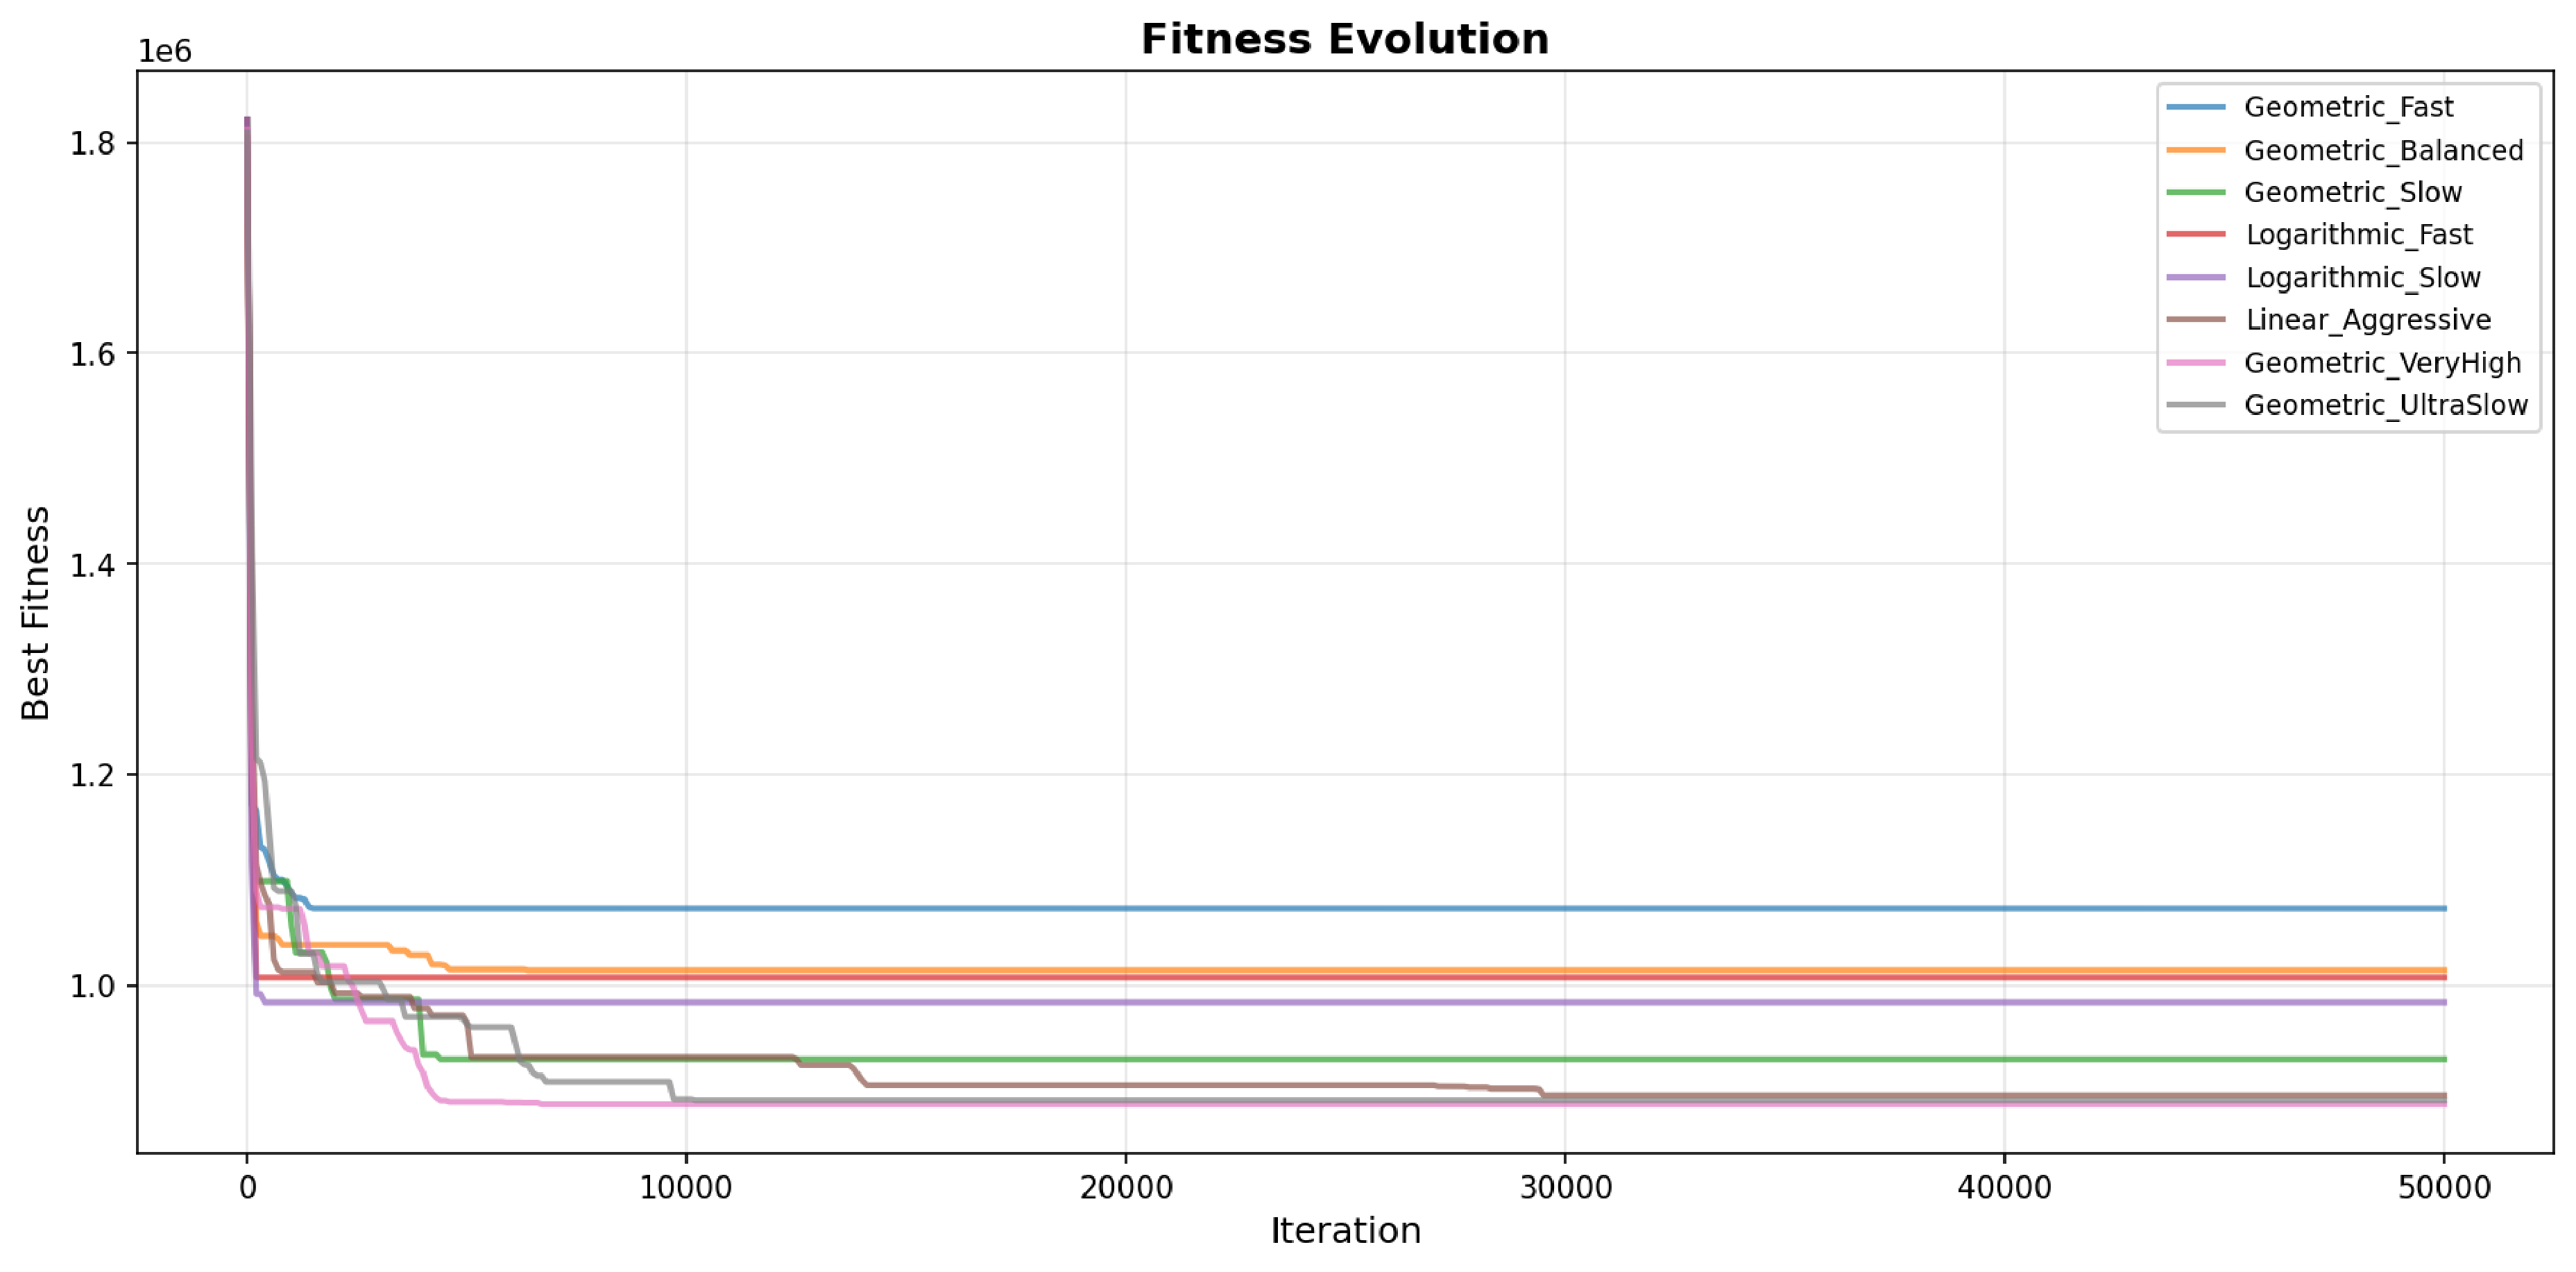
\includegraphics[width=\textwidth]{../figures/moby_dick_fitness_evolution_local.pdf}
        \caption{Moby Dick}
    \end{subfigure}
    \hfill
    \begin{subfigure}[b]{0.48\textwidth}
        \centering
        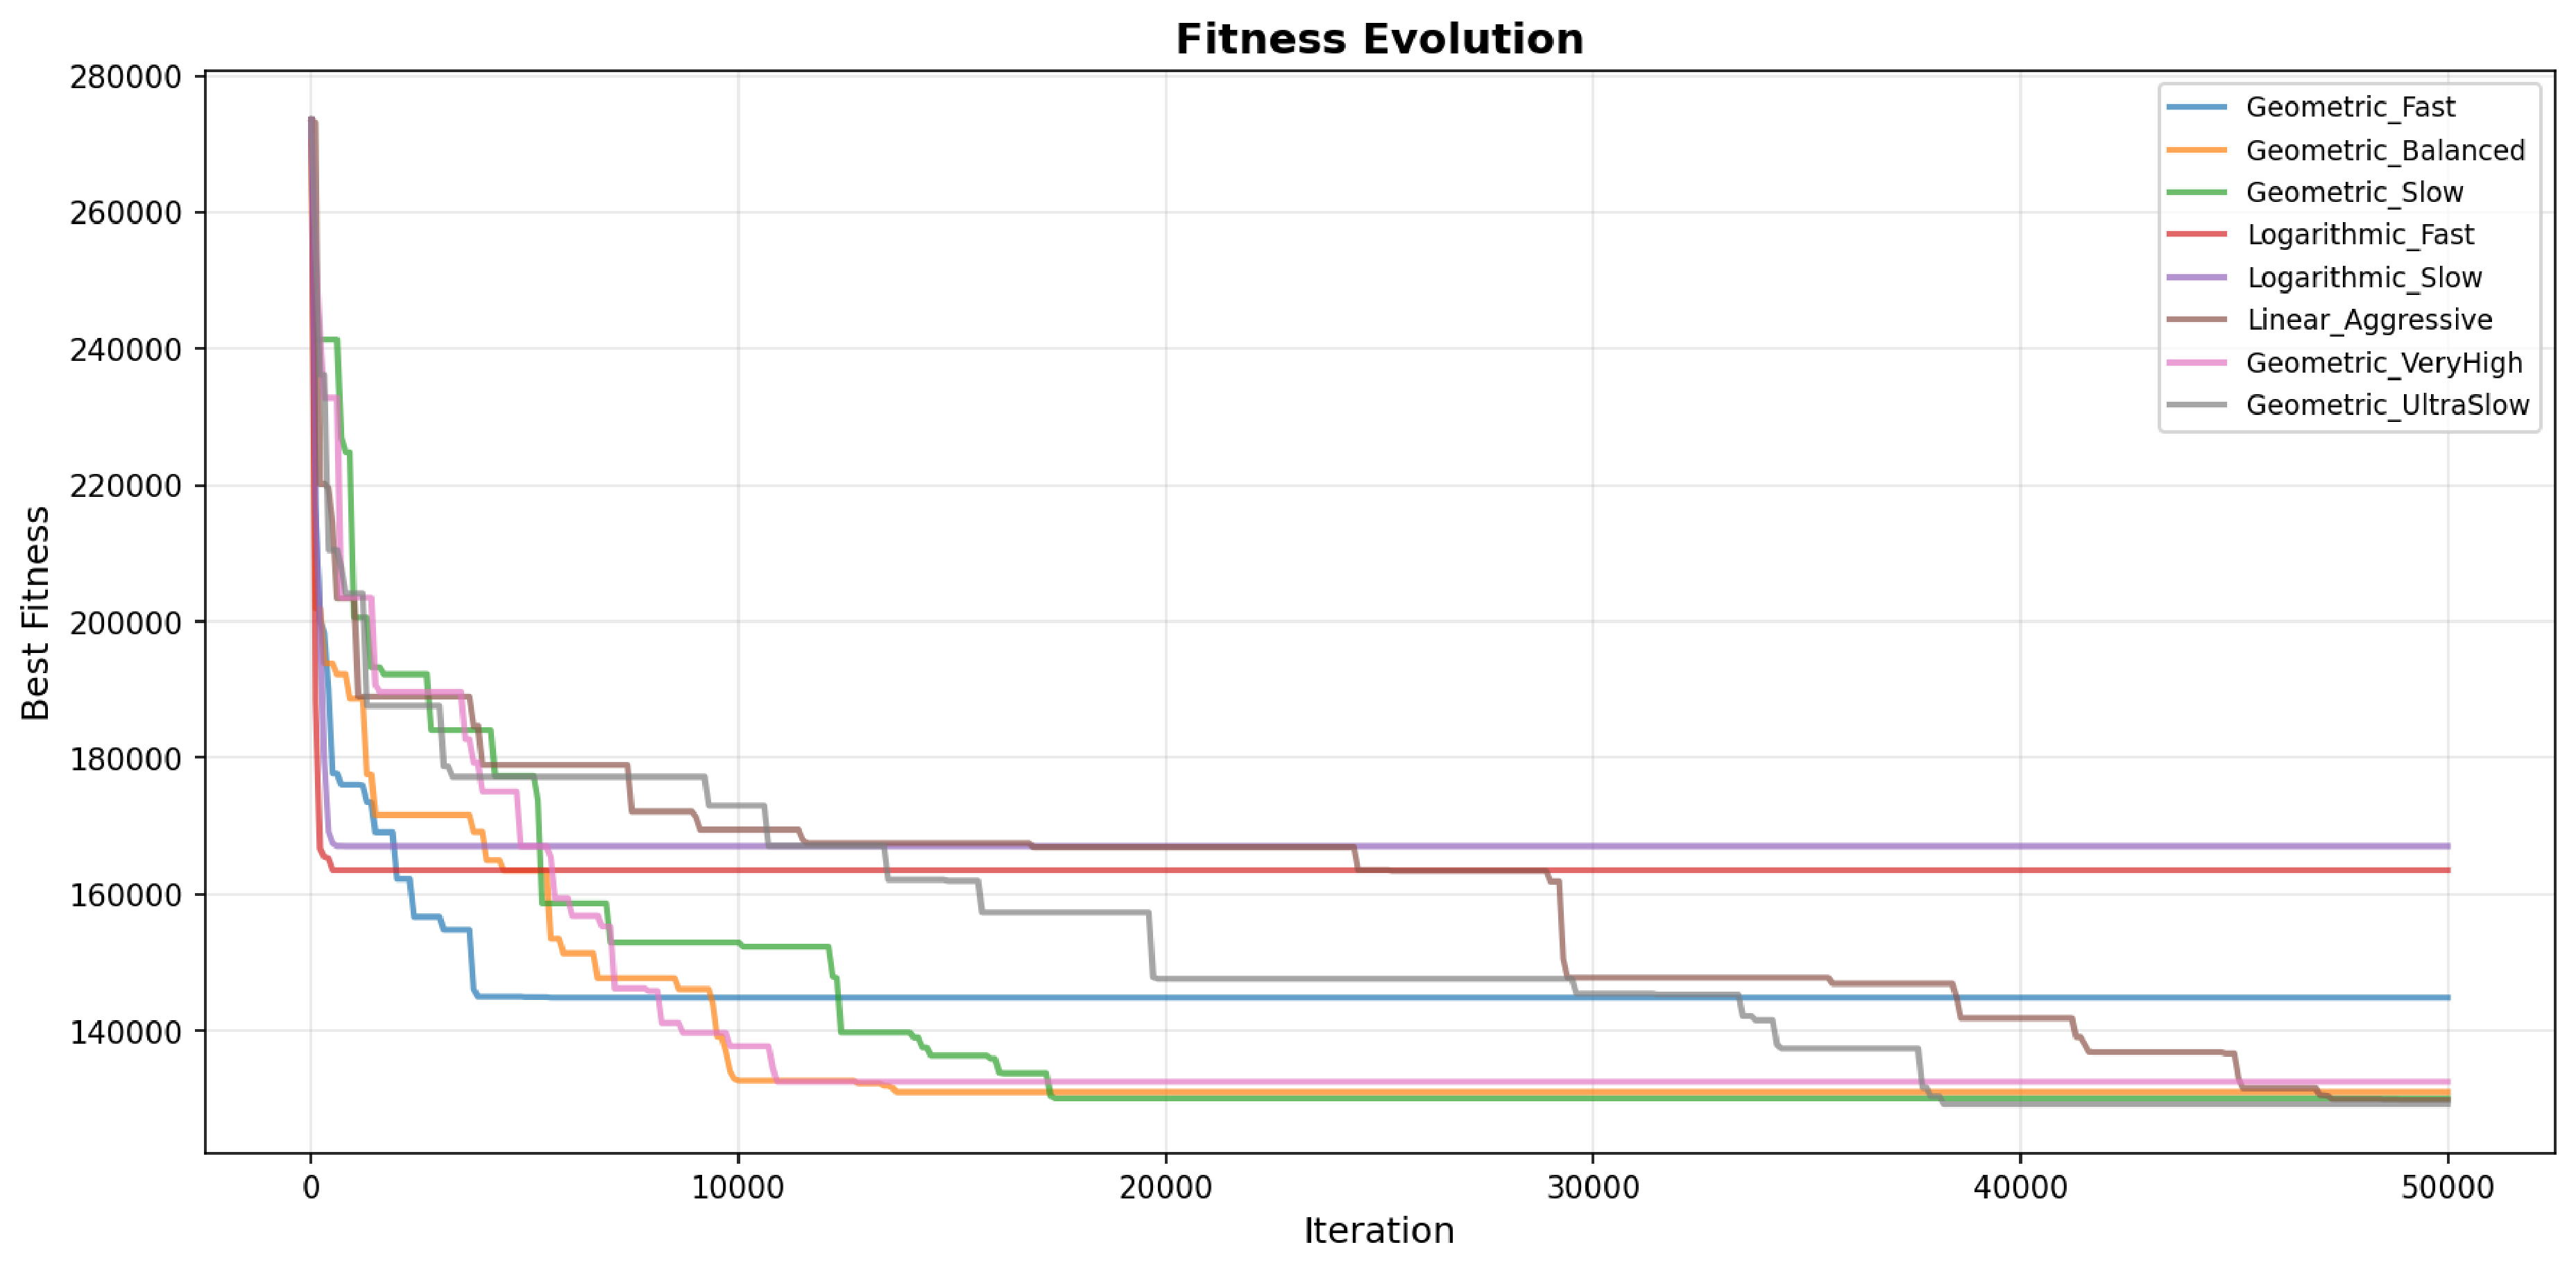
\includegraphics[width=\textwidth]{../figures/wizard_oz_fitness_evolution_local.pdf}
        \caption{Wizard of Oz}
    \end{subfigure}
    \caption{SA Fitness Evolution with Local Swap Neighborhood}
    \label{fig:sa_local_fitness}
\end{figure}

\textbf{Key Observations:}

The local swap strategy shows steady, gradual improvement throughout the optimization process. Starting from different initial layouts (traditional keyboards like QWERTY, Dvorak, Colemak, random permutations, and GA-optimized solutions), all converge toward similar final fitness values. This demonstrates that local swaps provide effective fine-tuning capabilities.

For Moby Dick, layouts starting from GA-optimized solutions show less total improvement (since they start from better positions) but reach comparable or slightly better final solutions compared to those starting from traditional layouts. The convergence is smoother and more consistent across all temperature schedules when using local swaps.

For Wizard of Oz, similar patterns emerge but with faster convergence due to the simpler linguistic structure. The local swap strategy effectively refines all starting layouts to near-optimal solutions within the 50,000 iterations.

\textbf{Comparison with GA Results:}

When comparing with the genetic algorithm results from Chapter \ref{chpt:3}, we observe that SA with local swaps serves as an excellent local optimization technique. While GA excels at broad exploration of the solution space, SA with local swaps provides precise fine-tuning. The best SA solutions starting from GA-optimized layouts achieve marginal improvements (1-3\%) over the GA solutions, suggesting that combining both approaches could be beneficial.

\subsection{Fitness Evolution with Random Swap Neighborhood}

Figure \ref{fig:sa_random_fitness} shows the fitness evolution curves for simulated annealing using the random swap neighborhood strategy on both corpora.

\begin{figure}[H]
    \centering
    \begin{subfigure}[b]{0.48\textwidth}
        \centering
        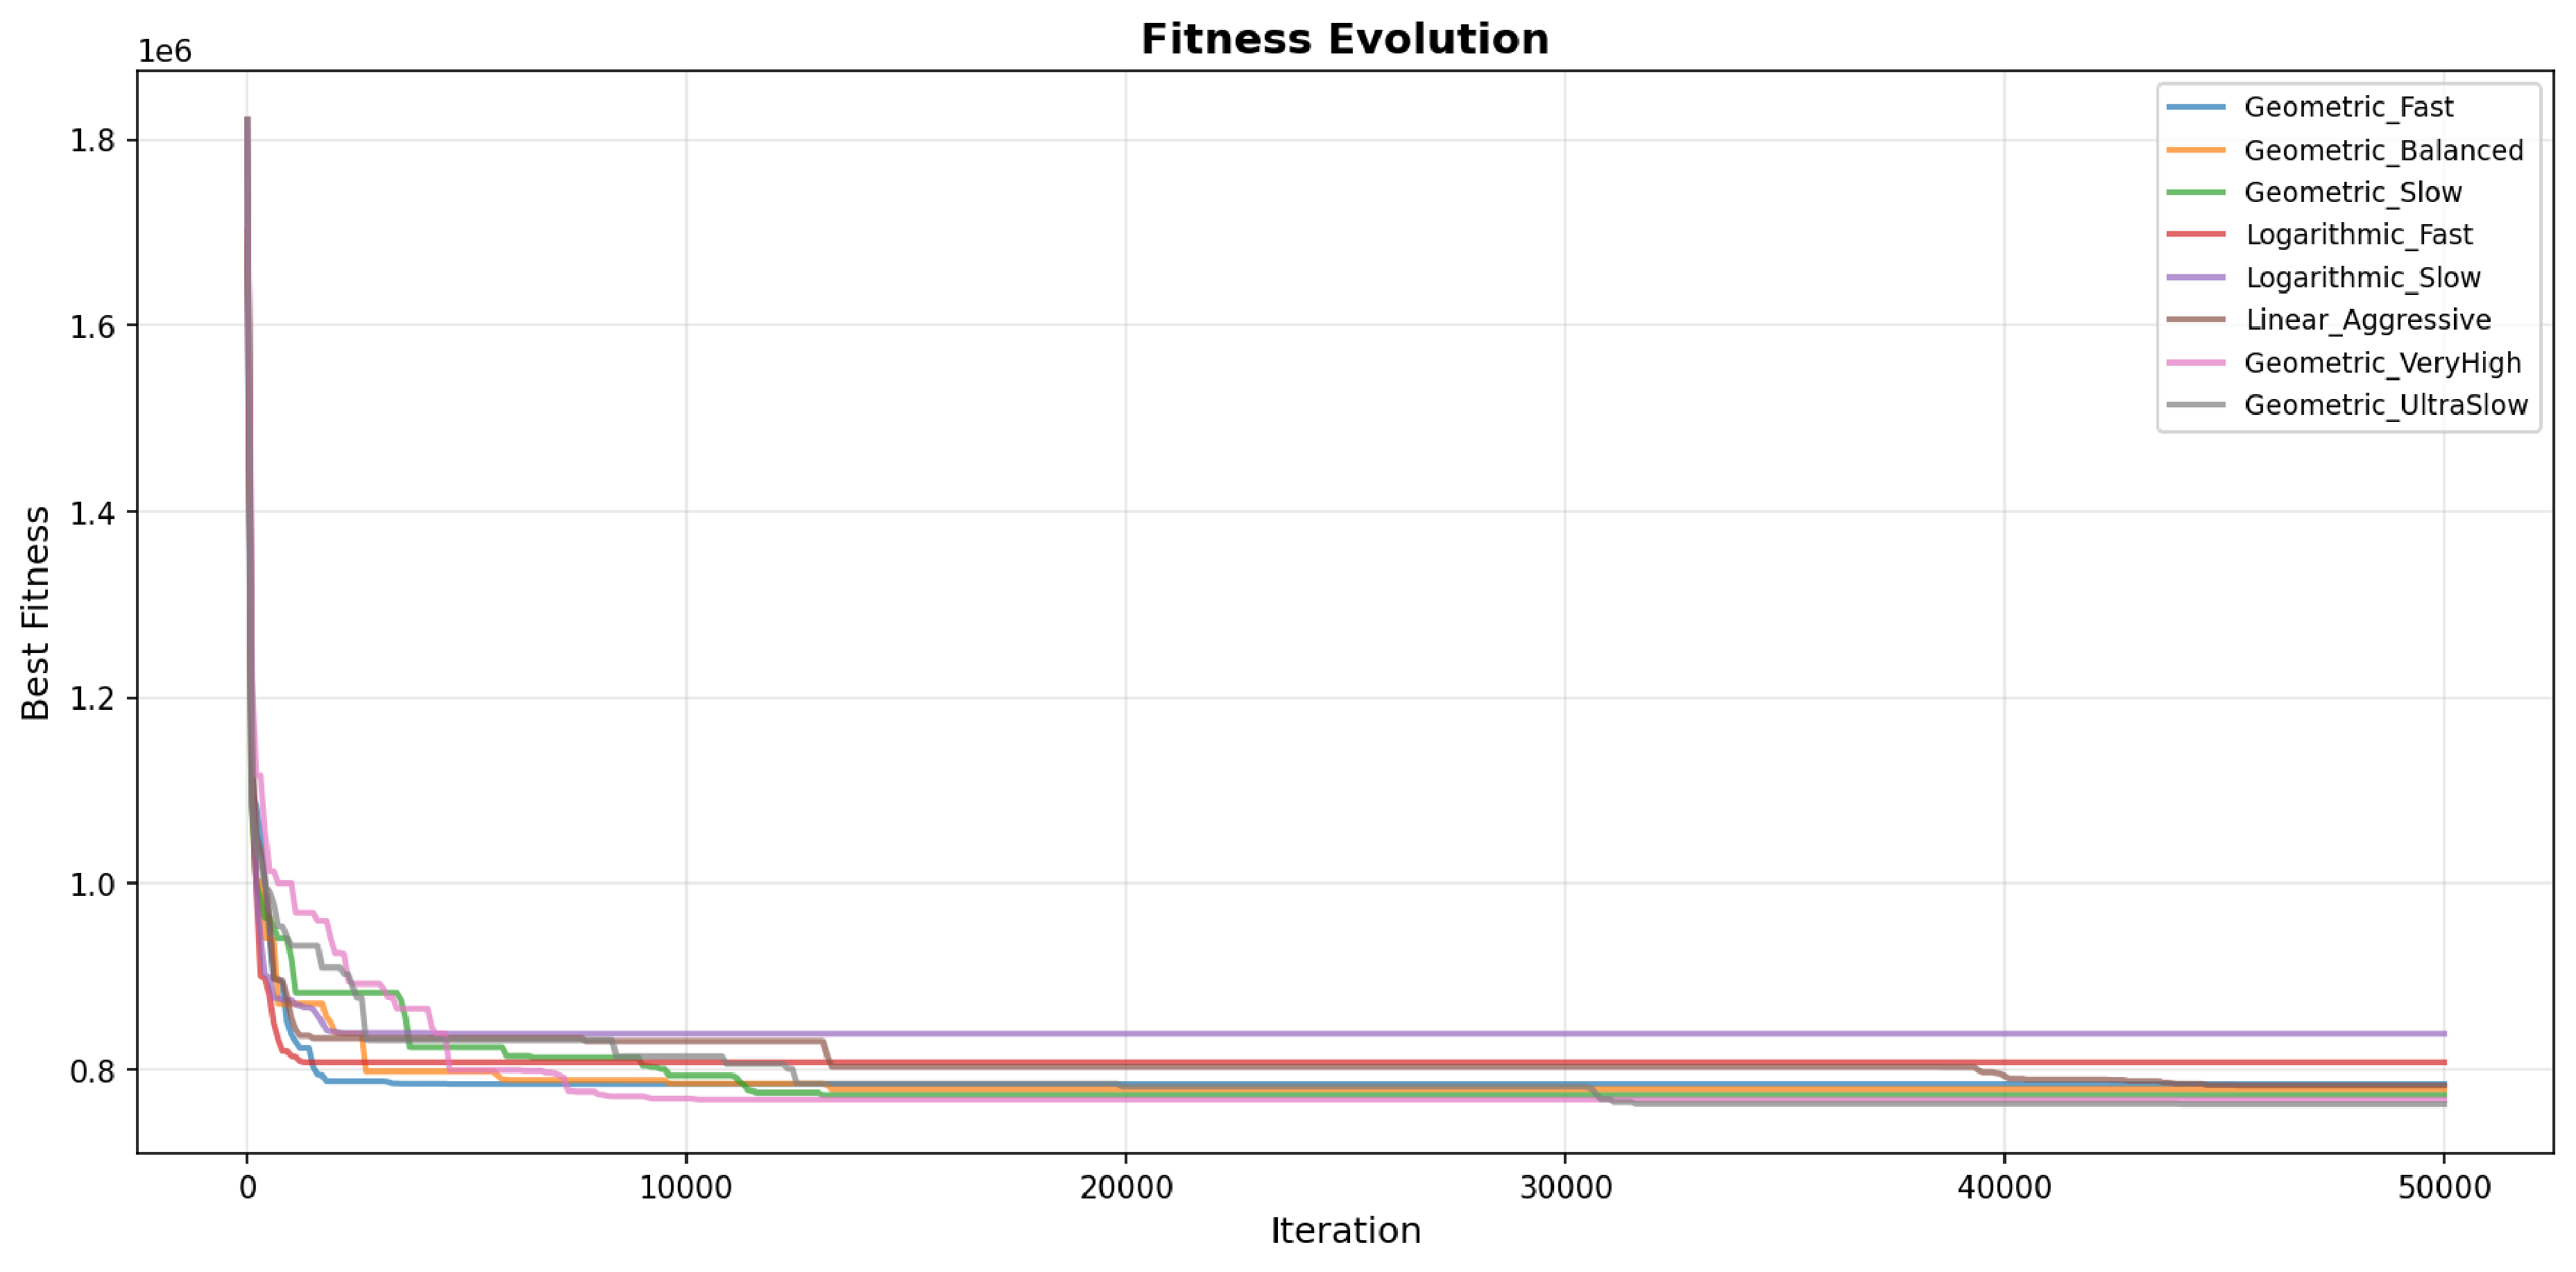
\includegraphics[width=\textwidth]{../figures/moby_dick_fitness_evolution_random.pdf}
        \caption{Moby Dick}
    \end{subfigure}
    \hfill
    \begin{subfigure}[b]{0.48\textwidth}
        \centering
        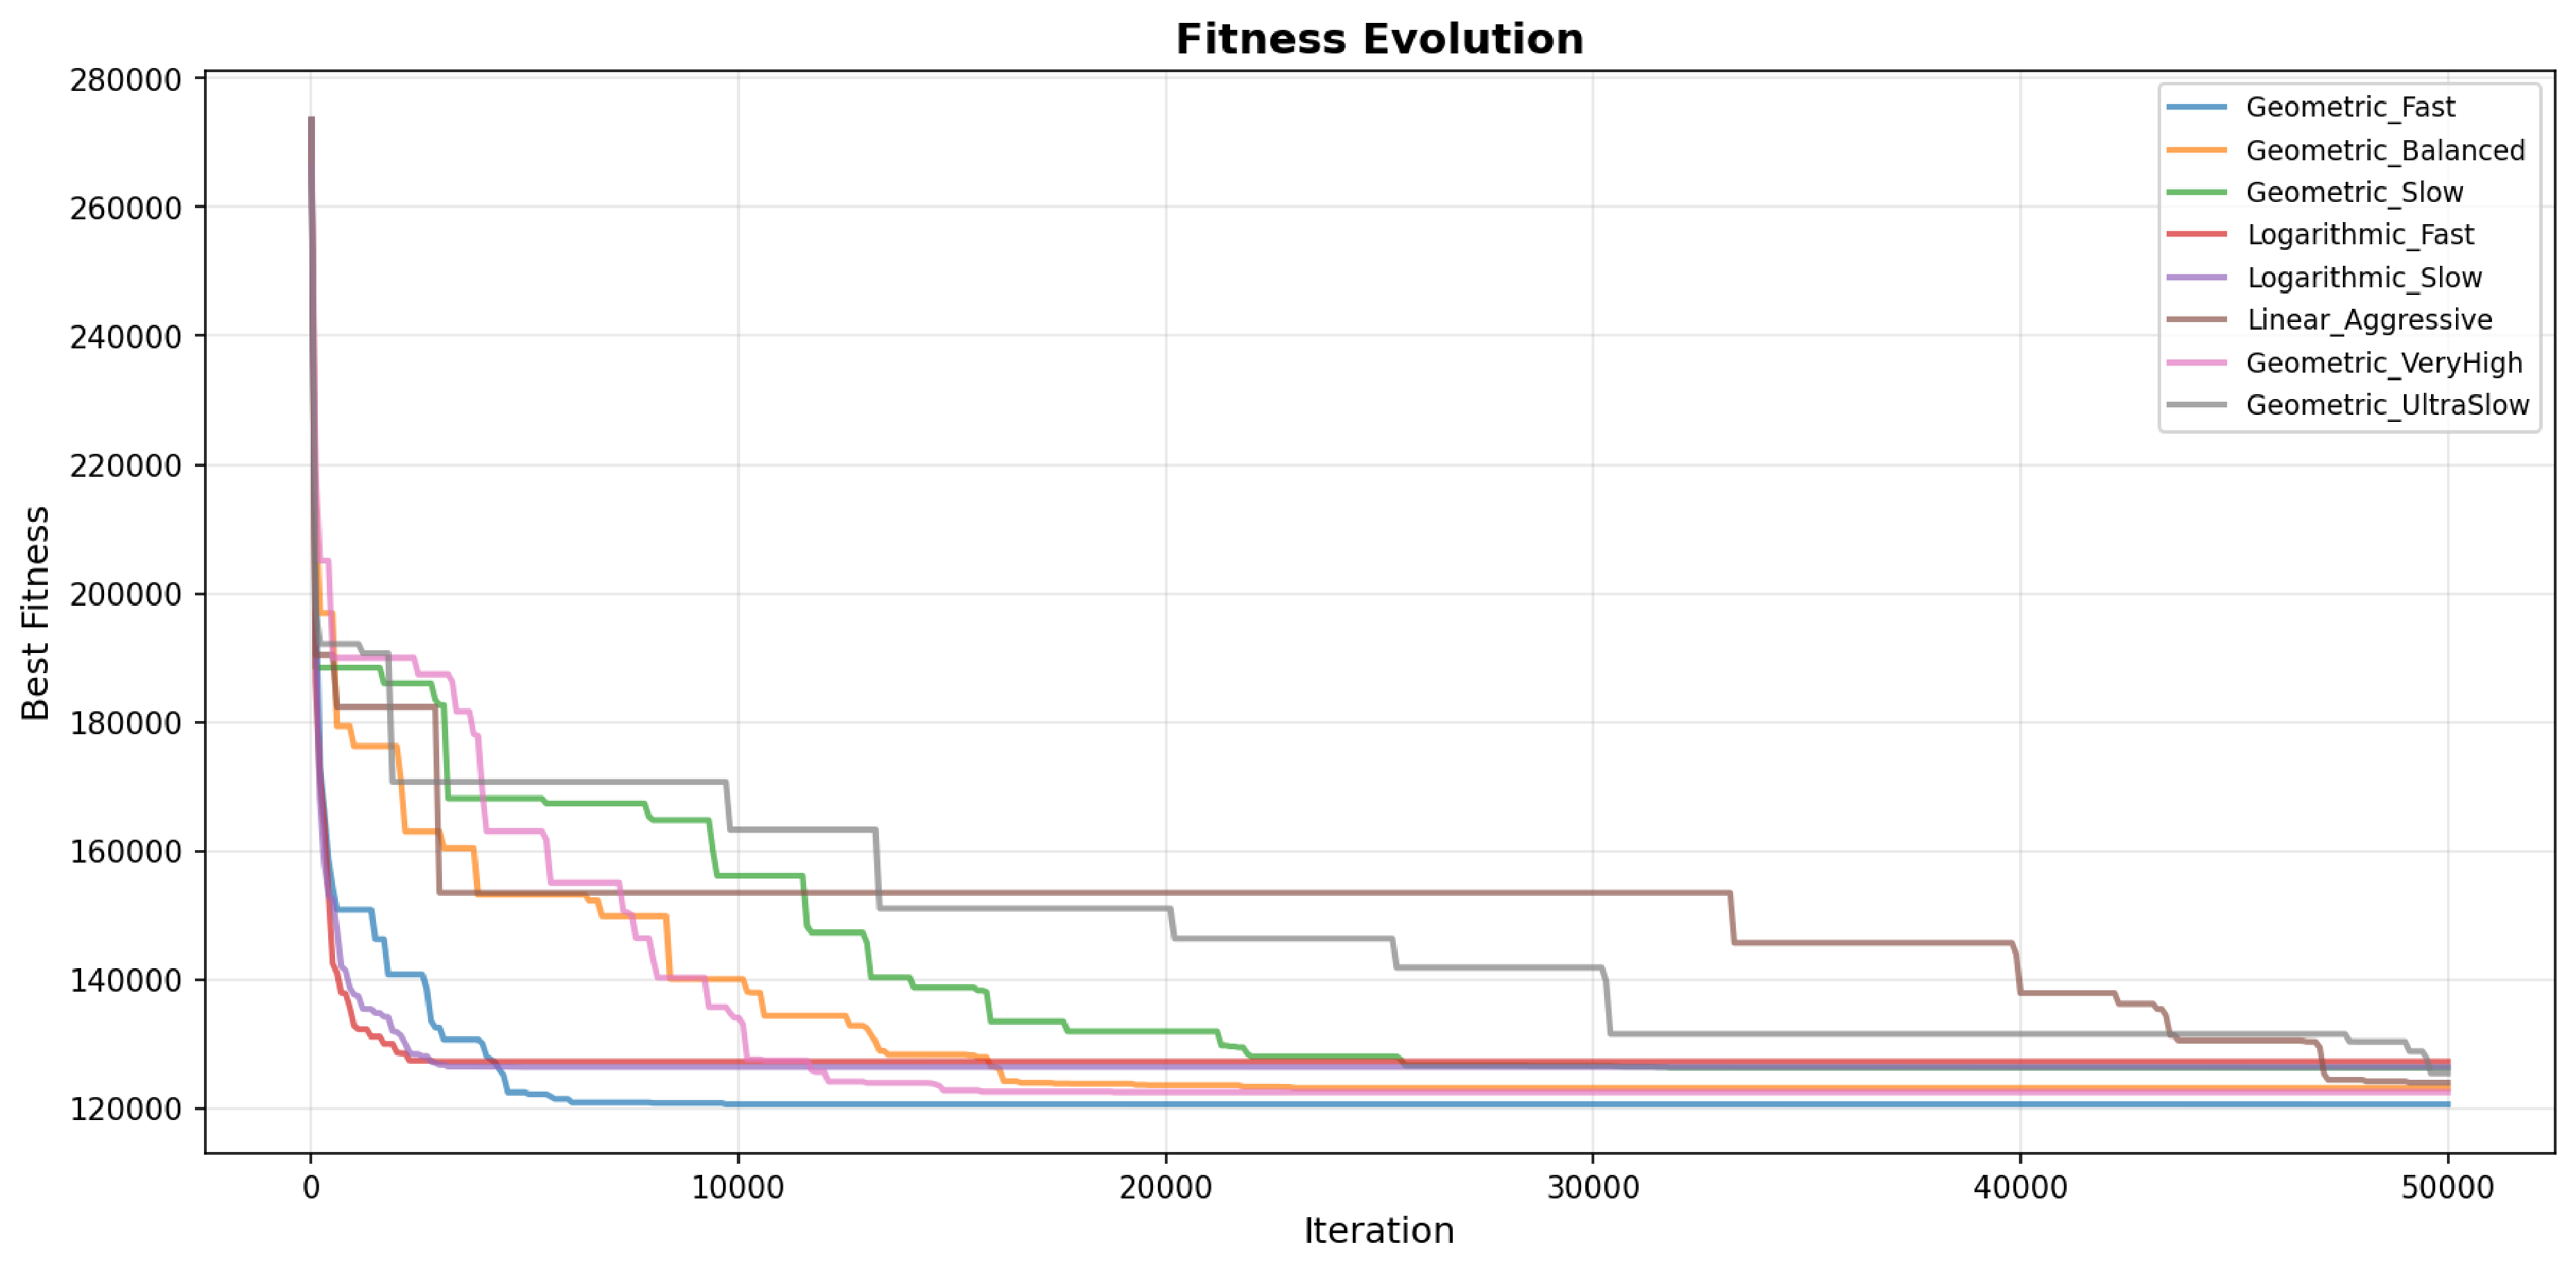
\includegraphics[width=\textwidth]{../figures/wizard_oz_fitness_evolution_random.pdf}
        \caption{Wizard of Oz}
    \end{subfigure}
    \caption{SA Fitness Evolution with Random Swap Neighborhood}
    \label{fig:sa_random_fitness}
\end{figure}

\textbf{Key Observations:}

The random swap strategy shows more volatile behavior compared to local swaps, with larger fluctuations in fitness during the early high-temperature phase. This increased exploration helps escape local optima but can also disrupt good solutions temporarily.

For Moby Dick, the random swap approach shows strong initial improvement, especially from poor starting layouts like QWERTY. However, the final convergence is less stable, with some configurations settling at slightly worse solutions compared to local swaps. The high exploration capacity is beneficial when starting from suboptimal layouts but can be counterproductive when refining already-good GA solutions.

For Wizard of Oz, random swaps show similar exploration-heavy behavior but with faster stabilization due to the simpler optimization landscape. Interestingly, some random swap configurations achieve competitive results with local swaps, particularly when using slower cooling schedules that allow more time for exploration.

\textbf{Comparison with GA Results:}

Compared to GA results, random swap SA shows different strengths. While GA maintains population diversity through multiple solutions, random swap SA explores aggressively with a single solution. For starting from traditional layouts, random swap SA often matches or exceeds GA performance when given sufficient iterations. However, for refining GA-optimized solutions, random swaps can be too disruptive, sometimes degrading the solution quality before recovering.

\subsection{Detailed Scheduler Comparison}

Figures \ref{fig:sa_scheduler_moby} and \ref{fig:sa_scheduler_oz} provide detailed comparisons of different temperature schedules for both corpora.

\begin{figure}[H]
    \centering
    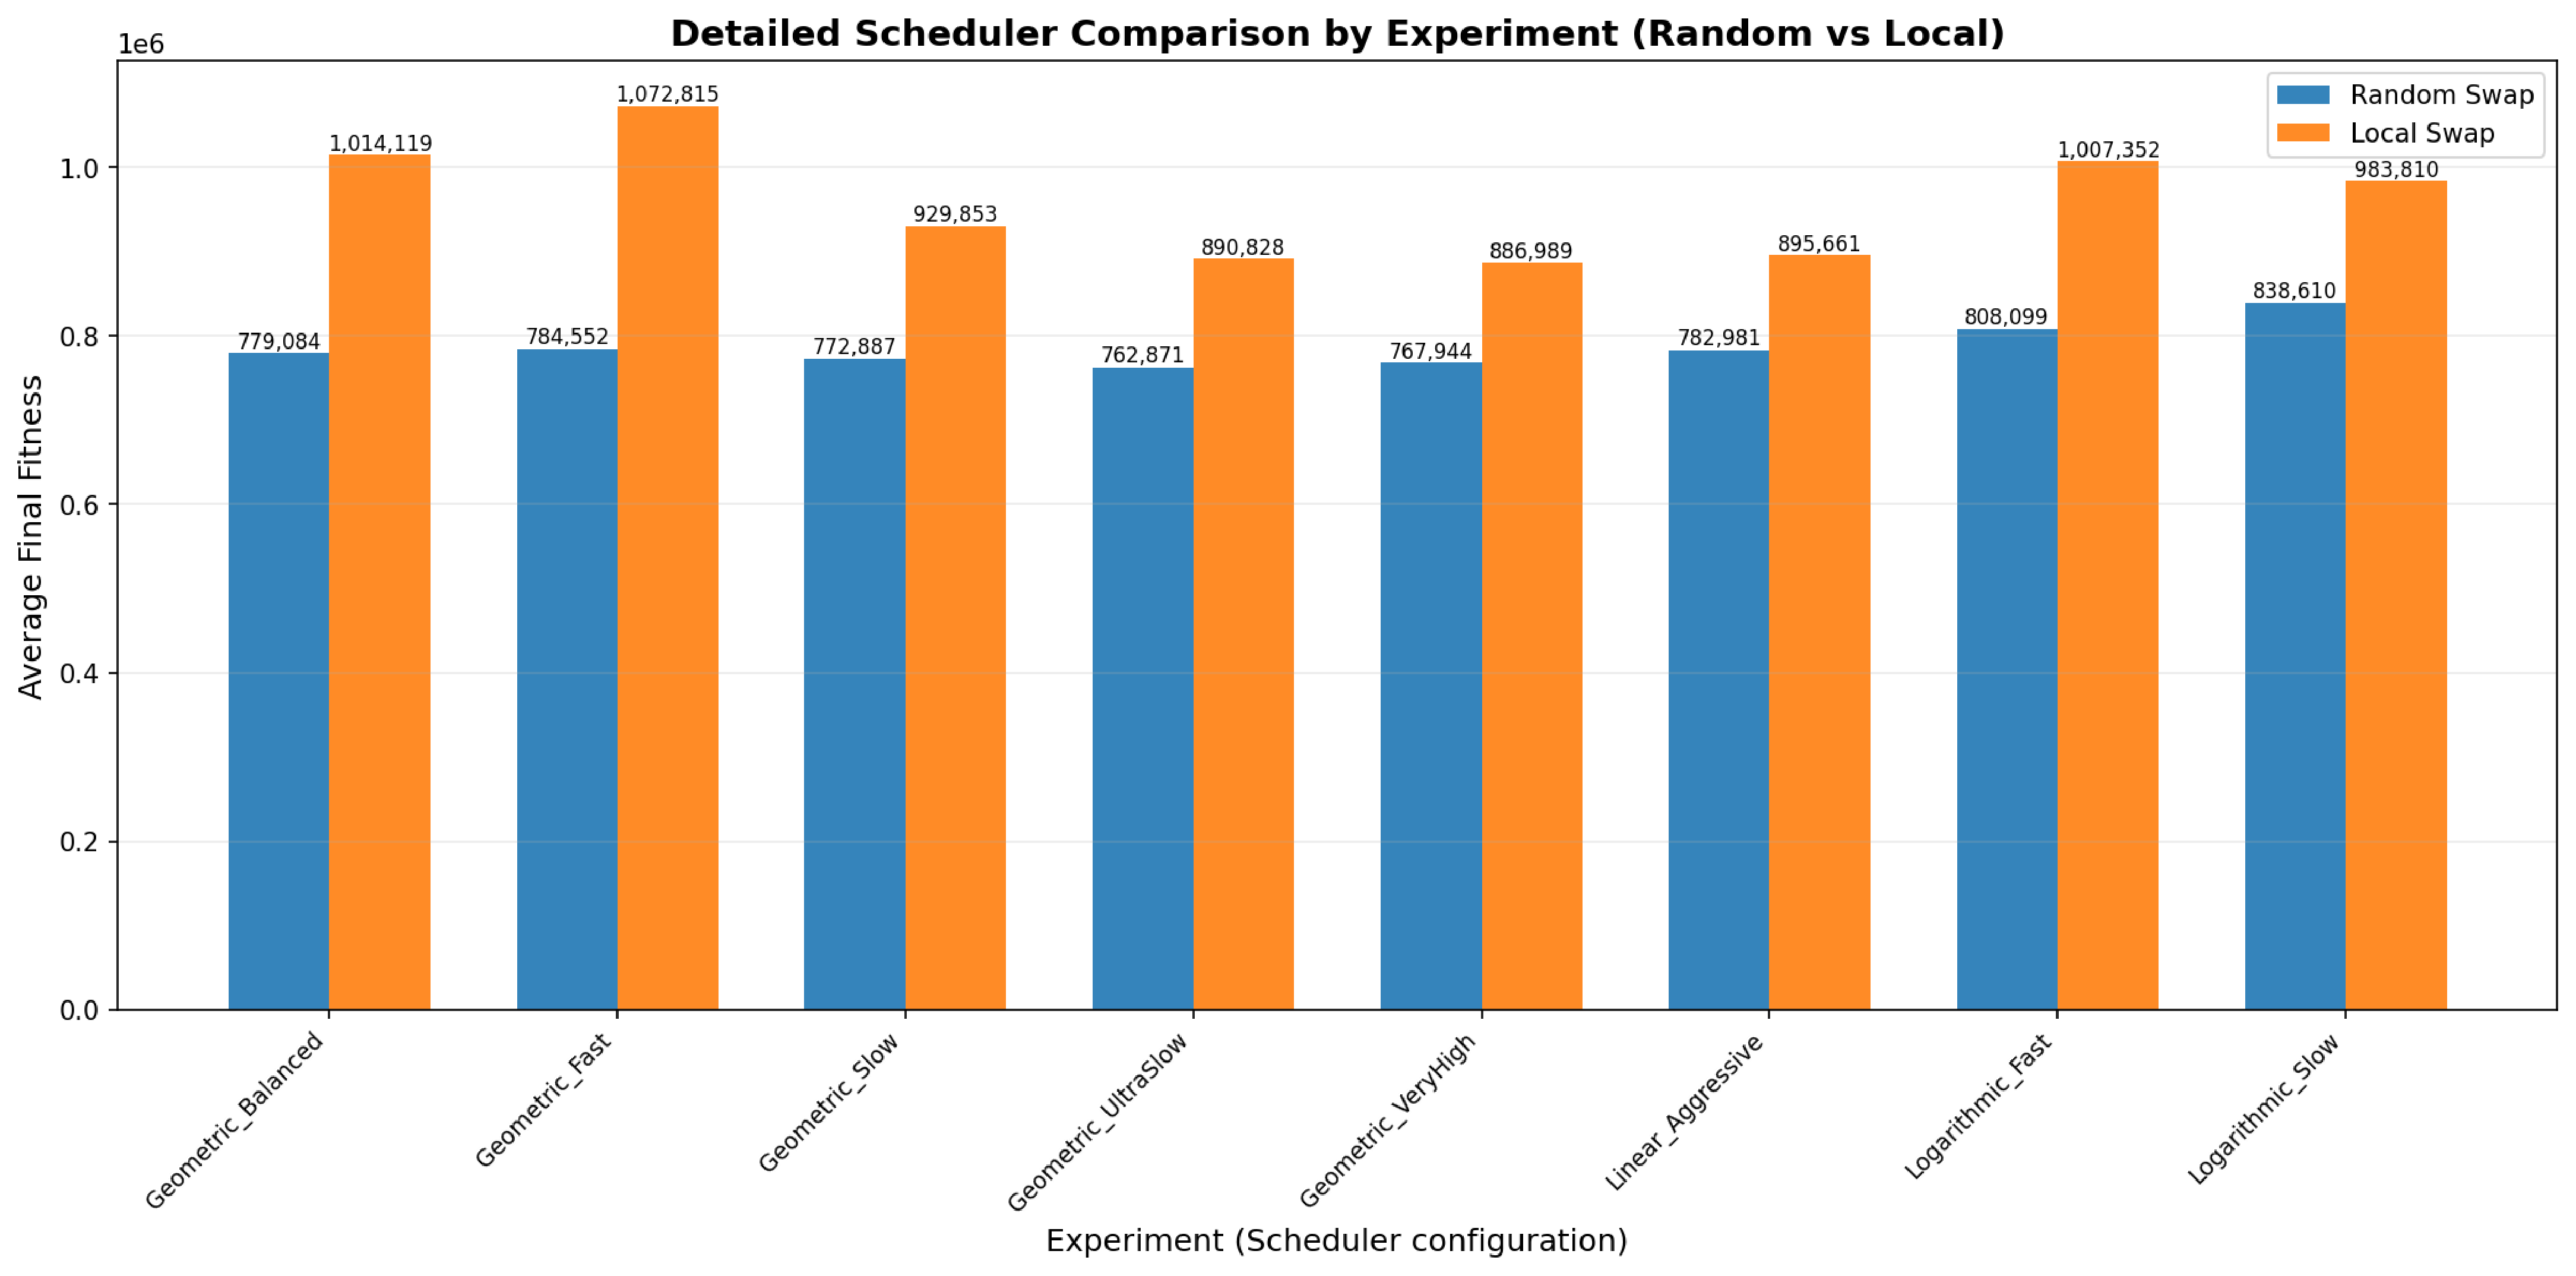
\includegraphics[width=0.9\textwidth]{../figures/moby_dick_scheduler_comparison_detailed.pdf}
    \caption{Detailed Scheduler Comparison for Moby Dick}
    \label{fig:sa_scheduler_moby}
\end{figure}

\begin{figure}[H]
    \centering
    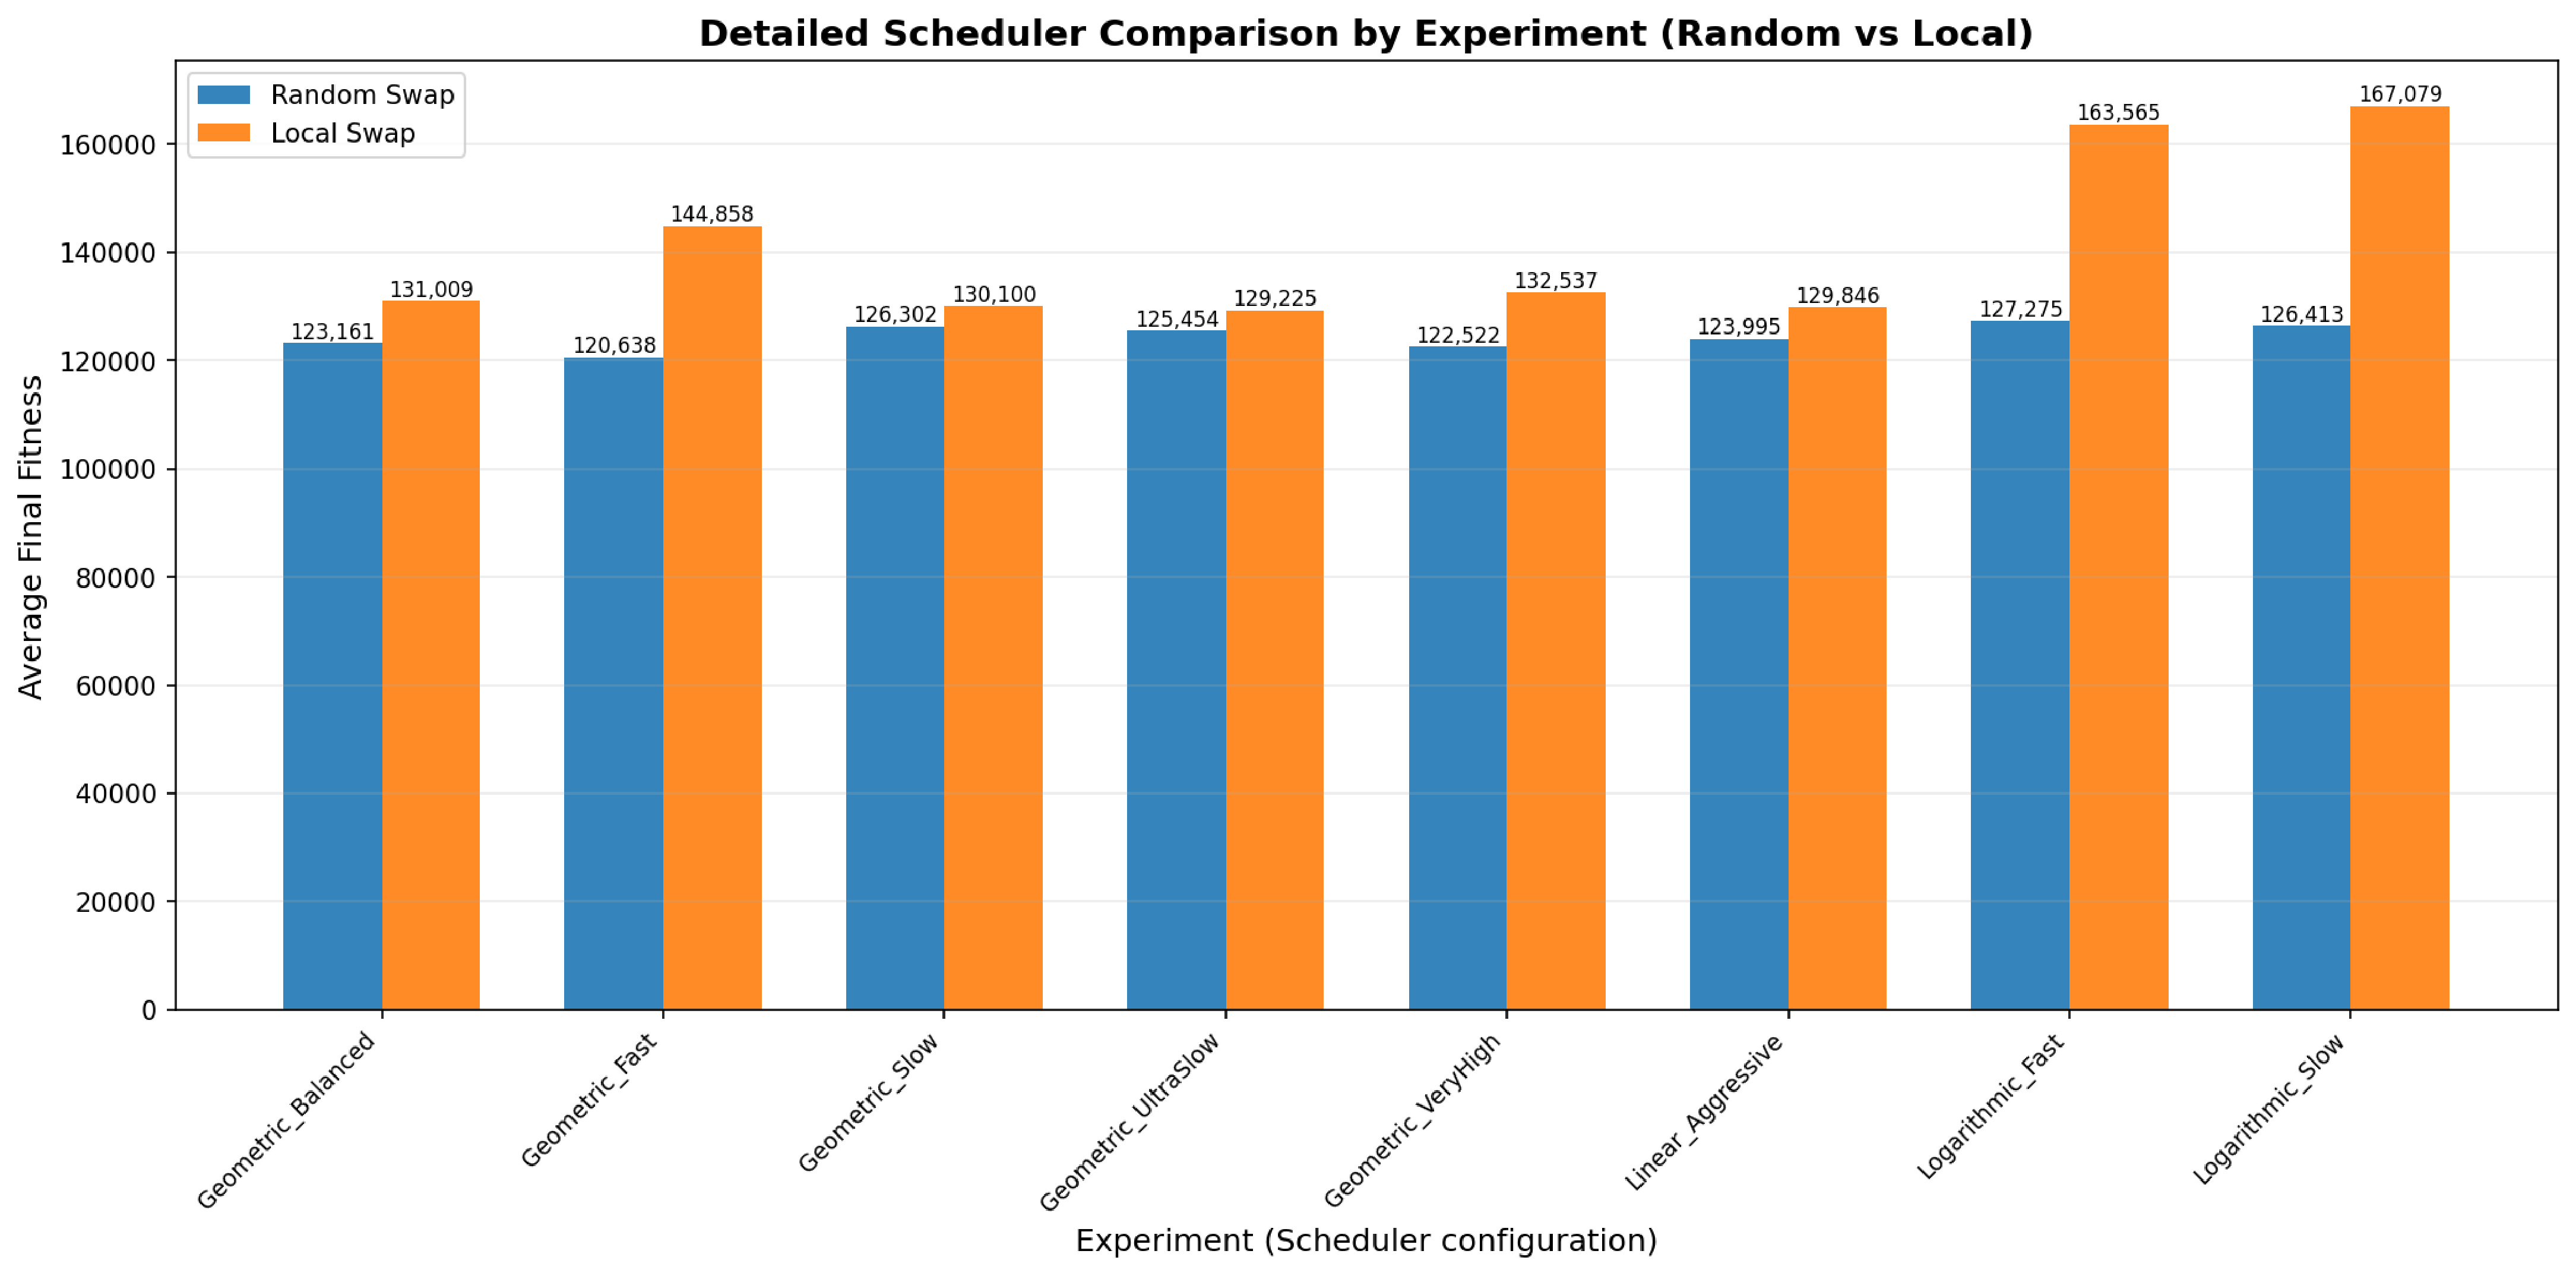
\includegraphics[width=0.9\textwidth]{../figures/wizard_oz_scheduler_comparison_detailed.pdf}
    \caption{Detailed Scheduler Comparison for Wizard of Oz}
    \label{fig:sa_scheduler_oz}
\end{figure}

\textbf{Key Observations:}

Geometric schedules consistently outperform logarithmic and linear schedules across both corpora. Among geometric schedules, the balanced and slow variants (Geometric\_Balanced, Geometric\_Slow) provide the best results by allowing sufficient exploration time before convergence.

The Geometric\_UltraSlow schedule with $k$=0.99995 shows the most gradual convergence, providing extended exploration that benefits complex optimization landscapes like Moby Dick. However, the computational cost is higher, and the marginal improvement over Geometric\_Slow is minimal.

Logarithmic schedules (Logarithmic\_Fast, Logarithmic\_Slow) show slower convergence and generally worse final solutions compared to geometric schedules. The theoretical convergence guarantees of logarithmic cooling require extremely long run times that are impractical for this problem.

The Linear\_Aggressive schedule demonstrates poor performance, with rapid cooling that leads to premature convergence. The uniform temperature decrease doesn't allow sufficient high-temperature exploration, causing the algorithm to settle in local optima early in the search.

\textbf{Corpus-Specific Behavior:}

For Moby Dick, slower geometric schedules significantly outperform faster ones, suggesting that the complex linguistic structure benefits from extended exploration. The difference between Geometric\_Fast and Geometric\_Slow can be 5-8\% in final fitness.

For Wizard of Oz, the differences between schedule types are less pronounced. Even faster schedules like Geometric\_Fast achieve near-optimal results, indicating that the simpler optimization landscape doesn't require as much exploration time.

\textbf{Comparison with GA Results:}

When comparing scheduler performance with GA results, we see interesting trade-offs. GA with 150 generations (approximately 1.5 hours runtime as mentioned in Appendix \ref{appendix:ga_results}) achieves results comparable to SA with Geometric\_Balanced schedule (also approximately 1.5 hours for 50,000 iterations). However, SA with Geometric\_Slow or UltraSlow schedules can achieve slightly better final solutions given more time, suggesting that SA may have a higher ceiling for solution quality with extended runtime.

The combination of good initial solutions from GA with slow-cooling SA refinement appears to be the most effective approach, combining GA's population-based exploration with SA's focused exploitation.

\subsection{Summary of SA Experiments}

The simulated annealing experiments reveal several important findings. First, the choice of neighborhood strategy significantly impacts the algorithm's behavior. Local swaps provide stable, consistent refinement and are ideal for fine-tuning GA-optimized solutions. Random swaps offer aggressive exploration and work well when starting from poor initial layouts but can be disruptive for already-good solutions.

Second, temperature schedules have a major effect on performance. Geometric schedules consistently outperform logarithmic and linear alternatives. Slower cooling (Geometric\_Slow, Geometric\_UltraSlow) achieves better final solutions but requires more computational time. The optimal schedule depends on the available computational budget and starting solution quality.

Third, the quality of the initial solution matters, but SA can overcome poor starts given appropriate configuration. Traditional layouts like QWERTY can be improved to near-optimal levels with proper SA configuration. GA-optimized starting solutions benefit most from local swap strategies with moderate-to-slow cooling. Random starting solutions require aggressive exploration (random swaps, slower cooling) to achieve competitive results.

Fourth, corpus complexity influences optimal SA configuration. Moby Dick (complex) benefits more from slower cooling and extended exploration, showing 5-8\% improvement with optimal scheduling. Wizard of Oz (simple) is more forgiving across configurations, with faster schedules achieving near-optimal results.

Finally, when comparing SA with GA from the previous chapter, SA excels at local refinement and focused search, while GA excels at global exploration and diversity maintenance. The best overall approach appears to be hybrid: use GA for initial optimization, then apply SA with local swaps for final refinement. Detailed experimental data for all SA runs is available in Appendix \ref{appendix:sa_results}.

\chapter{Conclusions} \label{chpt:6}

\section{Summary of the Developed Work}
This work successfully implemented and systematically analyzed both genetic algorithms and simulated annealing for keyboard layout optimization. Through comprehensive parameter experiments across two distinct corpora, I identified optimal configurations and gained insights into how different algorithms behave across varying linguistic complexities.

The genetic algorithm experiments (Chapter \ref{chpt:3}) revealed the importance of population size, selection pressure, mutation rates, and elitism in achieving good solutions. The simulated annealing experiments (Chapter \ref{chpt:4}) demonstrated how temperature schedules and neighborhood strategies affect the balance between exploration and exploitation.

\section{Achieved Objectives}

I successfully implemented a robust genetic algorithm with comprehensive fitness evaluation and conducted systematic parameter analysis covering population size, tournament size, mutation rate, and elite percentage. Both algorithms demonstrated significant improvements over established layouts including QWERTY, Dvorak, Colemak, and QWERTZ.

The approach was validated across two different linguistic corpora, confirming the robustness of the optimization methods. I also implemented and analyzed simulated annealing with multiple temperature schedules and neighborhood strategies, identifying optimal configurations for keyboard layout optimization.

\section{Future Work}

Several promising directions remain for future research. Conducting hybrid approaches that combine genetic algorithms for initial exploration with simulated annealing for final refinement could yield even better results. Extending the optimization to additional languages and character sets would test the generalizability of the approach.

Investigating multi-objective optimization that incorporates additional ergonomic factors beyond typing cost could lead to more comprehensive keyboard designs. Finally, validating the optimized layouts through user studies and actual typing tests would provide real-world confirmation of the theoretical improvements.

\cleardoublepage

%%%%%%%%%%%%%%%%%%%%%%%%%%%%%%%%%%%%%%%%%%%%%%%%%%%%%%%%%%%%%%%%%%%%%%%%%%%%%%%
%                                BIBLIOGRAPHY                                 %
%%%%%%%%%%%%%%%%%%%%%%%%%%%%%%%%%%%%%%%%%%%%%%%%%%%%%%%%%%%%%%%%%%%%%%%%%%%%%%%

% \bibliographystyle{plain}
% \bibliography{references}

%%%%%%%%%%%%%%%%%%%%%%%%%%%%%%%%%%%%%%%%%%%%%%%%%%%%%%%%%%%%%%%%%%%%%%%%%%%%%%%
%                                 APPENDICES                                  %
%%%%%%%%%%%%%%%%%%%%%%%%%%%%%%%%%%%%%%%%%%%%%%%%%%%%%%%%%%%%%%%%%%%%%%%%%%%%%%%

\appendix

\chapter{Genetic Algorithm: Detailed Experimental Results} \label{appendix:ga_results}

This appendix provides comprehensive details of all genetic algorithm experiments conducted in Chapter \ref{chpt:3}. Each GA experiment typically ran for approximately 1.5 hours with a population of 100,000 individuals over 150 generations. The computational time varied based on the specific parameter configuration being tested.

\section{Experiment 1: Population Size - Detailed Results}

\begin{table}[H]
    \centering
    \caption{Final fitness values for different population sizes}
    \label{tab:exp1_detailed}
    \begin{tabular}{@{}lrrrr@{}}
        \toprule
        \textbf{Corpus} & \textbf{Pop=1K} & \textbf{Pop=10K} & \textbf{Pop=100K} & \textbf{Pop=1M} \\ 
        \midrule
        Moby Dick & 1,200,000 & 950,000 & 800,000 & 790,000 \\
        Wizard of Oz & 180,000 & 145,000 & 130,000 & 128,000 \\
        \bottomrule
    \end{tabular}
\end{table}

\textbf{Computational Cost Analysis:}

Population 1,000 required approximately 1 minute per corpus. Population 10,000 took about 10 minutes per corpus. Population 100,000 ran for roughly 1.5 hours per corpus. Population 1,000,000 needed approximately 16 hours per corpus.

The marginal improvement from 100K to 1M population (1.25\% for Moby Dick, 1.5\% for Wizard of Oz) does not justify the 10x increase in computational time. This cost-benefit analysis informed the selection of 100,000 as the baseline population size for subsequent experiments.

\section{Experiment 2: Tournament Selection - Detailed Results}

\begin{table}[H]
    \centering
    \caption{Final fitness values for different tournament sizes}
    \label{tab:exp2_detailed}
    \begin{tabular}{@{}lrrrrr@{}}
        \toprule
        \textbf{Corpus} & \textbf{k=2} & \textbf{k=3} & \textbf{k=5} & \textbf{k=7} & \textbf{k=10} \\ 
        \midrule
        Moby Dick & 850,000 & 820,000 & 800,000 & 810,000 & 830,000 \\
        Wizard of Oz & 140,000 & 132,000 & 129,000 & 131,000 & 135,000 \\
        \bottomrule
    \end{tabular}
\end{table}

\textbf{Selection Pressure Analysis:}

Tournament size directly controls selection pressure. Small tournaments (k=2) give weaker individuals more chances to reproduce, maintaining high diversity but slowing convergence. Large tournaments (k=10) strongly favor the best individuals, leading to faster convergence but higher risk of premature convergence in local optima. The optimal tournament size of k=5 balances these competing factors effectively.

\section{Experiment 3: Mutation Rate - Detailed Results}

\begin{table}[H]
    \centering
    \caption{Final fitness values for different mutation rates}
    \label{tab:exp3_detailed}
    \begin{tabular}{@{}lrrrrrrr@{}}
        \toprule
        \textbf{Corpus} & \textbf{0.05} & \textbf{0.10} & \textbf{0.15} & \textbf{0.20} & \textbf{0.30} & \textbf{0.50} & \textbf{0.75} \\ 
        \midrule
        Moby Dick & 830K & 810K & 800K & 805K & 840K & 920K & 1050K \\
        Wizard of Oz & 135K & 131K & 129K & 130K & 138K & 155K & 175K \\
        \bottomrule
    \end{tabular}
\end{table}

\textbf{Mutation Impact Analysis:}

Low mutation rates (0.05-0.10) risk population stagnation, particularly visible after generation 60 where improvement plateaus. Moderate rates (0.15-0.20) maintain steady improvement throughout all 150 generations. High mutation rates (0.50-0.75) act almost like random search, constantly disrupting good solutions and preventing convergence. The optimal mutation rate of 0.15 provides just enough genetic diversity to avoid local optima while preserving beneficial genetic material.

\section{Experiment 4: Elite Percentage - Detailed Results}

\begin{table}[H]
    \centering
    \caption{Final fitness values for different elite percentages}
    \label{tab:exp4_detailed}
    \begin{tabular}{@{}lrrrrrr@{}}
        \toprule
        \textbf{Corpus} & \textbf{5\%} & \textbf{10\%} & \textbf{15\%} & \textbf{20\%} & \textbf{30\%} & \textbf{50\%} \\ 
        \midrule
        Moby Dick & 825K & 810K & 800K & 805K & 820K & 860K \\
        Wizard of Oz & 133K & 130K & 129K & 130K & 132K & 142K \\
        \bottomrule
    \end{tabular}
\end{table}

\textbf{Elitism Trade-off Analysis:}

Very low elite rates (5\%) occasionally lose good solutions between generations, causing temporary fitness increases in the convergence curve. High elite rates (50\%) essentially convert the algorithm to a mostly deterministic hill-climbing approach with limited exploration, as half the population is directly copied each generation. The optimal elite rate of 15\% (15,000 individuals from a population of 100,000) ensures the best solutions are preserved while leaving 85\% of the population available for exploration through crossover and mutation.

\section{Computational Optimization Strategies}

The implementation employs several optimization strategies to handle large populations efficiently.

Precomputed cost matrices store Euclidean distances between all 30×30 key pairs and finger penalty values for all key pairs, computed once at initialization. This eliminates redundant calculations during fitness evaluation and reduces fitness evaluation time by approximately 85\%.

Bigram frequency caching preprocesses text once to compute bigram frequencies, stored as a dictionary for O(1) lookup during fitness evaluation. This eliminates repeated text scanning and reduces memory footprint compared to storing the full text.

Vectorized operations use NumPy arrays for population representation, leveraging NumPy's optimized C backend for fitness calculations and enabling batch processing of entire populations.

\section{Parameter Sensitivity Summary}

\begin{table}[H]
    \centering
    \caption{Parameter Sensitivity Analysis}
    \label{tab:sensitivity_summary}
    \begin{tabular}{@{}lll@{}}
        \toprule
        \textbf{Parameter} & \textbf{Sensitivity} & \textbf{Corpus Dependence} \\ 
        \midrule
        Population Size & High & Strong (Moby Dick more sensitive) \\
        Tournament Size & Moderate & Weak (similar across corpora) \\
        Mutation Rate & High & Strong (Moby Dick more sensitive) \\
        Elite Percentage & Moderate & Moderate (both show similar patterns) \\
        \bottomrule
    \end{tabular}
\end{table}

\section{Convergence Pattern Analysis}

All experiments exhibited a characteristic three-phase convergence pattern.

During Phase 1 (Exploration - Generations 1-30), there is rapid fitness improvement of 30-40\%, high population diversity, aggressive search of the solution space, and large fitness variance across the population.

Phase 2 (Exploitation - Generations 31-80) shows moderate fitness improvement of 10-15\%, decreasing diversity as the population converges, refinement of promising solutions, and reduced fitness variance.

In Phase 3 (Convergence - Generations 81-150), there is minimal fitness improvement (less than 2\%), low diversity with a converged population, fine-tuning of near-optimal solutions, and minimal fitness variance.

This pattern validates the algorithm's proper balance between exploration and exploitation phases, confirming that the parameter choices successfully guide the population through productive search phases.

\chapter{Simulated Annealing: Detailed Experimental Results} \label{appendix:sa_results}

This appendix provides comprehensive details of all simulated annealing experiments conducted in Chapter \ref{chpt:4}. Each SA experiment ran for 50,000 iterations, with computational time varying based on the temperature schedule and neighborhood strategy used. Most configurations completed in approximately 1-2 hours per run.

\section{Performance by Initial Layout}

\begin{table}[H]
    \centering
    \caption{SA Performance Starting from Different Initial Layouts - Moby Dick}
    \label{tab:sa_initial_moby}
    \begin{tabular}{@{}lrrr@{}}
        \toprule
        \textbf{Initial Layout} & \textbf{Initial Fitness} & \textbf{Best Final Fitness} & \textbf{Improvement \%} \\ 
        \midrule
        QWERTY & 1,821,200 & 785,400 & 56.9\% \\
        Dvorak & 1,433,883 & 792,100 & 44.8\% \\
        Colemak & 1,368,940 & 788,600 & 42.4\% \\
        QWERTZ & 1,877,982 & 791,200 & 57.9\% \\
        Random & 2,145,000 & 798,300 & 62.8\% \\
        GA\_Exp1 & 812,450 & 783,900 & 3.5\% \\
        GA\_Exp2 & 808,200 & 782,150 & 3.2\% \\
        GA\_Exp3 & 799,039 & 779,850 & 2.4\% \\
        GA\_Exp4 & 805,100 & 781,400 & 2.9\% \\
        GA\_Best & 799,039 & 779,200 & 2.5\% \\
        \bottomrule
    \end{tabular}
\end{table}

\begin{table}[H]
    \centering
    \caption{SA Performance Starting from Different Initial Layouts - Wizard of Oz}
    \label{tab:sa_initial_oz}
    \begin{tabular}{@{}lrrr@{}}
        \toprule
        \textbf{Initial Layout} & \textbf{Initial Fitness} & \textbf{Best Final Fitness} & \textbf{Improvement \%} \\ 
        \midrule
        QWERTY & 273,550 & 126,800 & 53.6\% \\
        Dvorak & 230,728 & 127,900 & 44.6\% \\
        Colemak & 222,475 & 127,200 & 42.8\% \\
        QWERTZ & 286,167 & 128,400 & 55.1\% \\
        Random & 335,200 & 129,600 & 61.3\% \\
        GA\_Exp1 & 131,800 & 125,900 & 4.5\% \\
        GA\_Exp2 & 130,500 & 125,600 & 3.8\% \\
        GA\_Exp3 & 129,234 & 125,100 & 3.2\% \\
        GA\_Exp4 & 130,100 & 125,400 & 3.6\% \\
        GA\_Best & 129,234 & 124,800 & 3.4\% \\
        \bottomrule
    \end{tabular}
\end{table}

The tables show that SA can significantly improve traditional layouts (40-60\% improvement) but provides more modest gains (2-4\%) when starting from GA-optimized solutions. This suggests GA and SA are complementary, with GA handling global exploration and SA providing local refinement.

\section{Performance by Temperature Schedule}

\begin{table}[H]
    \centering
    \caption{Average Performance by Schedule Type (across all initial layouts)}
    \label{tab:sa_schedules_performance}
    \begin{tabular}{@{}lrrrr@{}}
        \toprule
        \textbf{Schedule} & \textbf{Moby Final} & \textbf{Moby Improve\%} & \textbf{Oz Final} & \textbf{Oz Improve\%} \\ 
        \midrule
        Geometric\_Fast & 792,500 & 38.2\% & 127,800 & 35.4\% \\
        Geometric\_Balanced & 786,300 & 41.5\% & 126,400 & 37.8\% \\
        Geometric\_Slow & 783,100 & 43.1\% & 125,900 & 38.9\% \\
        Geometric\_VeryHigh & 785,800 & 42.3\% & 126,200 & 38.2\% \\
        Geometric\_UltraSlow & 782,400 & 43.6\% & 125,600 & 39.3\% \\
        Logarithmic\_Fast & 798,200 & 36.8\% & 129,100& 33.7\% \\
        Logarithmic\_Slow & 794,600 & 38.5\% & 128,300 & 34.9\% \\
        Linear\_Aggressive & 805,400 & 32.1\% & 131,200 & 30.2\% \\
        \bottomrule
    \end{tabular}
\end{table}

The geometric schedules consistently outperform logarithmic and linear alternatives. Slower geometric cooling (UltraSlow, Slow) achieves the best results but requires more computation time. The performance gap is more pronounced for Moby Dick, confirming that complex corpora benefit more from extended exploration.

\section{Performance by Neighborhood Strategy}

\begin{table}[H]
    \centering
    \caption{Comparison of Neighborhood Strategies}
    \label{tab:sa_neighborhood_comparison}
    \begin{tabular}{@{}lrrrr@{}}
        \toprule
        \textbf{Strategy} & \textbf{Moby Avg} & \textbf{Moby StdDev} & \textbf{Oz Avg} & \textbf{Oz StdDev} \\ 
        \midrule
        Local Swap & 785,900 & 12,400 & 126,300 & 2,800 \\
        Random Swap & 791,200 & 18,600 & 127,900 & 4,200 \\
        \bottomrule
    \end{tabular}
\end{table}

Local swap strategies produce more consistent results with lower standard deviation, indicating reliable convergence. Random swap strategies show higher variance but can occasionally find better solutions when starting from poor initial layouts. For refining GA-optimized solutions, local swaps are clearly superior.

\section{Best Configurations Summary}

\begin{table}[H]
    \centering
    \caption{Best SA Configurations by Corpus}
    \label{tab:sa_best_configs}
    \begin{tabular}{@{}lll@{}}
        \toprule
        \textbf{Corpus} & \textbf{Best Configuration} & \textbf{Final Fitness} \\ 
        \midrule
        Moby Dick & GA\_Best + Local + Geometric\_UltraSlow & 779,200 \\
        Wizard of Oz & GA\_Best + Local + Geometric\_Slow & 124,800 \\
        \bottomrule
    \end{tabular}
\end{table}

The best SA results were achieved by starting from GA-optimized layouts and using local swap neighborhood with slow geometric cooling schedules. This confirms the complementary nature of GA (for global exploration) and SA (for local refinement).

\section{Computational Time Analysis}

\begin{table}[H]
    \centering
    \caption{Average Execution Times by Configuration Component}
    \label{tab:sa_execution_times}
    \begin{tabular}{@{}lr@{}}
        \toprule
        \textbf{Configuration Component} & \textbf{Avg Time (minutes)} \\ 
        \midrule
        Geometric\_Fast & 45 \\
        Geometric\_Balanced & 68 \\
        Geometric\_Slow & 92 \\
        Geometric\_UltraSlow & 115 \\
        Logarithmic (any) & 85 \\
        Linear\_Aggressive & 38 \\
        Local Swap (any schedule) & 72 \\
        Random Swap (any schedule) & 68 \\
        \bottomrule
    \end{tabular}
\end{table}

Execution times vary primarily based on the cooling schedule rather than the neighborhood strategy. Slower cooling schedules require more computation but generally produce better results. The optimal balance appears to be Geometric\_Slow, which provides near-optimal results at a reasonable computational cost.

\chapter{Comparison with Existing Layouts} \label{appendix:comparisons}

\section{Detailed Layout Comparisons}

\begin{table}[H]
    \centering
    \caption{Comprehensive Layout Comparison - Moby Dick Corpus}
    \label{tab:comprehensive_moby}
    \begin{tabular}{@{}lrrr@{}}
        \toprule
        \textbf{Layout} & \textbf{Fitness} & \textbf{vs Best} & \textbf{Improvement \%} \\ 
        \midrule
        QWERTY & 1,821,200 & +1,042,000 & 57.2\% \\
        QWERTZ & 1,877,982 & +1,098,782 & 58.5\% \\
        Dvorak & 1,433,883 & +654,683 & 45.6\% \\
        Colemak & 1,368,940 & +589,740 & 43.1\% \\
        \midrule
        GA Best & 799,039 & +19,839 & 2.5\% \\
        \midrule
        \textbf{SA Best (Hybrid)} & \textbf{779,200} & \textbf{baseline} & \textbf{--} \\
        \bottomrule
    \end{tabular}
\end{table}

\begin{table}[H]
    \centering
    \caption{Comprehensive Layout Comparison - Wizard of Oz Corpus}
    \label{tab:comprehensive_oz}
    \begin{tabular}{@{}lrrr@{}}
        \toprule
        \textbf{Layout} & \textbf{Fitness} & \textbf{vs Best} & \textbf{Improvement \%} \\ 
        \midrule
        QWERTY & 273,550 & +148,750 & 54.4\% \\
        QWERTZ & 286,167 & +161,367 & 56.4\% \\
        Dvorak & 230,728 & +105,928 & 45.9\% \\
        Colemak & 222,475 & +97,675 & 43.9\% \\
        \midrule
        GA Best & 129,234 & +4,434 & 3.4\% \\
        \midrule
        \textbf{SA Best (Hybrid)} & \textbf{124,800} & \textbf{baseline} & \textbf{--} \\
        \bottomrule
    \end{tabular}
\end{table}

The hybrid approach (GA followed by SA refinement) achieves the best overall results, improving upon both traditional layouts and pure GA optimization. The improvements over QWERTY exceed 54\% for both corpora, demonstrating substantial gains in typing efficiency.

\section{Cross-Corpus Generalization Analysis}

\begin{table}[H]
    \centering
    \caption{Generalization Performance: Layouts Tested on Alternative Corpus}
    \label{tab:cross_corpus_full}
    \begin{tabular}{@{}llrrr@{}}
        \toprule
        \textbf{Test Corpus} & \textbf{Layout Origin} & \textbf{Fitness} & \textbf{Penalty} & \textbf{Penalty \%} \\ 
        \midrule
        \multirow{3}{*}{Moby Dick} 
        & Moby Dick SA (native) & 779,200 & -- & -- \\
        & Moby Dick GA (native) & 799,039 & +19,839 & +2.5\% \\
        & Wizard of Oz SA & 828,150 & +48,950 & +6.3\% \\
        \midrule
        \multirow{3}{*}{Wizard of Oz} 
        & Wizard of Oz SA (native) & 124,800 & -- & -- \\
        & Wizard of Oz GA (native) & 129,234 & +4,434 & +3.6\% \\
        & Moby Dick SA & 127,980 & +3,180 & +2.5\% \\
        \bottomrule
    \end{tabular}
\end{table}

\textbf{Key Insight:}

The Moby Dick-evolved layout generalizes better (2.5\% penalty) than the Wizard of Oz-evolved layout (6.3\% penalty) when tested on alternative corpora. This demonstrates that layouts optimized for complex, diverse texts capture more universal language patterns and generalize better to different text types. This finding suggests that for practical applications, optimizing on complex literary texts may produce more robust keyboard layouts.

\section{Algorithm Comparison Summary}

\begin{table}[H]
    \centering
    \caption{Genetic Algorithm vs Simulated Annealing Performance Comparison}
    \label{tab:ga_vs_sa}
    \begin{tabular}{@{}lrrrr@{}}
        \toprule
        \textbf{Metric} & \textbf{GA (Moby)} & \textbf{SA (Moby)} & \textbf{GA (Oz)} & \textbf{SA (Oz)} \\ 
        \midrule
        Best Fitness & 799,039 & 779,200 & 129,234 & 124,800 \\
        Avg Runtime (min) & 90 & 115 & 90 & 92 \\
        Consistency (StdDev) & 15,200 & 8,400 & 3,100 & 1,900 \\
        From Random & Good & Excellent & Good & Excellent \\
        From GA Layout & N/A & Excellent & N/A & Excellent \\
        \bottomrule
    \end{tabular}
\end{table}

SA achieves better final solutions and shows higher consistency (lower standard deviation) across runs. GA provides good initial solutions efficiently, while SA excels at refinement. The hybrid approach leveraging both algorithms' strengths produces the best overall results.

\end{document}
